
\label{sec:apendice}

El apéndice reúne el material de apoyo que el cuerpo del documento cita: la reproducción del procesamiento, el linaje de las tablas, los nombres de las variables, el catálogo de covariables y las tablas y figuras complementarias de cada etapa de los Resultados.

%--------------------------------------------------------------------------------------
\anexo{Disponibilidad de datos y código, y reproducción}
\label{app:reproducibilidad}

Esta sección indica dónde están los datos y el código y cómo se repite el procesamiento; la cita la Sección~\ref{sec:metodologia}.

Las cuatro fuentes son públicas: los microdatos de la GEIH y el anexo de mercado laboral se descargan del archivo nacional de datos del DANE, TerriData del portal del DNP y la DIVIPOLA del geoportal del DANE (Tabla~\ref{tab:fuentes_datos}). El código está en el repositorio \url{https://github.com/juanp001/Estimacion-desempleo-Colombia-SAE}. Todo corre en Databricks con tablas de Unity Catalog en el catálogo \texttt{tesis} y se despliega como un conjunto de trabajos programados. Con el entorno configurado, el procesamiento completo se repite con el trabajo \texttt{pipeline\_completo}, que recibe el año y el mes de cierre y el número de meses de la ventana.

La Tabla~\ref{tab:app_jobs} relaciona cada trabajo con sus tareas y con las etapas de la metodología que cubre. El trabajo del modelo escribe también las tablas de la comparación entre el Fay-Herriot espacial y el clásico que usa la Sección~\ref{sec:res_espacial}: el SEBLUP de los 23 dominios con su ECM, su CV y su peso, las diferencias entre las dos estimaciones en dominios y municipios, y el índice de Moran de las 83 estimaciones municipales. Las dos figuras de esa comparación y el mapa municipal no salen de los trabajos: las dibuja el guion \texttt{img/\_script/figuras\_resultados.py}, versionado junto con el documento, que lee esas tablas sin recalcular ninguna cifra.

Las cifras del documento corresponden a la corrida del 31 de octubre de 2026 de la ingesta y el preprocesamiento y a la del 5 de noviembre de 2026 del análisis y el modelo, con la versión del repositorio etiquetada \texttt{documento-v1}.

\begin{table}[!htbp]
\centering
\small
\caption[Trabajos programados del procesamiento]{Trabajos programados del procesamiento y etapas de la metodología que cubren. La sensibilidad a la ventana temporal (etapa 5) se ejecuta aparte. GEIH: Gran Encuesta Integrada de Hogares; DANE: Departamento Administrativo Nacional de Estadística; DIVIPOLA: División Político-Administrativa de Colombia.}
\label{tab:app_jobs}
\begin{adjustbox}{max width=\linewidth}
\begin{tabular}{l p{8.6cm} l}
\toprule
Trabajo & Tareas & Etapas \\
\midrule
dimensiones & Tabla de la DIVIPOLA; dominios de la GEIH y sus municipios; capitales con coordenadas & 4 \\
ingesta\_geih & Capas bronce, plata y oro de la GEIH; cifras publicadas por el DANE & 1, 2 \\
ingesta\_terridata & Capas bronce y plata de TerriData; diccionario de indicadores & 1, 2 \\
preprocesamiento & Estimación directa; covariables por dominio y auditoría; pre-filtrado; municipios objetivo & 5 a 7 \\
analisis & Análisis descriptivo; selección de covariables y su sensibilidad al umbral $q$ & 8, 9 \\
modelo & Fay-Herriot clásico; Fay-Herriot espacial y tablas de su comparación con el clásico; sensibilidad a la varianza & 10 a 16 \\
pipeline\_completo & Ejecuta los seis trabajos anteriores en orden & 1 a 16 \\
\midrule
\multicolumn{3}{l}{Fuera de los trabajos} \\
\texttt{figuras\_resultados.py} & Figuras de la comparación espacial y mapa de los 83 municipios, a partir de las tablas del trabajo del modelo & 13, 16 \\
\bottomrule
\end{tabular}
\end{adjustbox}
\end{table}
%--------------------------------------------------------------------------------------
\anexo{Linaje de tablas}
\label{app:linaje}

Esta sección relaciona cada tabla del procesamiento con el cuaderno que la escribe y la etapa de la metodología; la citan las Secciones~\ref{sec:metodologia} y~\ref{sec:resultados}.

La Tabla~\ref{tab:app_linaje} se lee de arriba abajo en el orden en que corre el procesamiento: las capas de la GEIH y de TerriData alimentan la estimación directa y las covariables, y estas al modelo, que escribe la tabla final. Con ella se puede ubicar el cuaderno que produce cada cifra de los Resultados.

{\footnotesize\setlength{\tabcolsep}{3pt}
\begin{longtable}{p{2.8cm} p{3.6cm} p{4.8cm} p{1.2cm}}
\caption[Linaje de las tablas del procesamiento]{Linaje de las tablas del catálogo de Unity Catalog del trabajo, de la ingesta a la tabla final. GEIH: Gran Encuesta Integrada de Hogares; DIVIPOLA: División Político-Administrativa de Colombia; EBLUP: mejor predictor lineal insesgado empírico; GVF: función generalizada de varianza.}
\label{tab:app_linaje} \\
\toprule
Esquema & Contenido & Cuaderno & Etapa \\
\midrule
\endfirsthead
\multicolumn{4}{l}{\tablename~\thetable{}, continuación} \\
\toprule
Esquema & Contenido & Cuaderno & Etapa \\
\midrule
\endhead
\bottomrule
\endlastfoot
\texttt{geih\_bronce} & Un archivo por módulo y sección (cabecera y resto del marco antiguo; un archivo por módulo en el marco nuevo) y el factor de expansión recalculado & \texttt{geih\_bronce} & 1 \\
\texttt{geih\_bronce} & Cifras publicadas: nacionales, por ciudad (trimestre móvil) y anuales & \texttt{datos\_publicados} & 1 \\
\texttt{geih\_plata} & Un módulo consolidado por tabla (características generales, fuerza de trabajo, ocupados, no ocupados) y factores de expansión & \texttt{geih\_plata} & 2 \\
\texttt{geih\_oro} & Mercado laboral (una fila por persona); llaves sin pareja; reconciliación de la fuerza de trabajo & \texttt{geih\_oro} & 2 \\
\texttt{terridata} & Indicadores en formato largo (bronce) y ancho (plata) & \texttt{terridata\_bronce, terridata\_plata} & 1, 2 \\
\texttt{dim} & DIVIPOLA; dominios de la GEIH; capitales con coordenadas; diccionario de indicadores & \texttt{dim\_divipola, dim\_dominio\_geih, dim\_geih\_divipola, terridata\_plata} & 1, 4 \\
\texttt{preprocesamiento} & Tasa directa por dominio; sensibilidad de la ventana & \texttt{estimacion\_directa, sensibilidad\_ventana\_temporal} & 5 \\
\texttt{preprocesamiento} & Tasa con covariables; reglas de agregación; auditoría de dominios & \texttt{adicion\_covariables} & 4, 6 \\
\texttt{preprocesamiento} & Covariables pre-filtradas; cascada; sensibilidad de la variabilidad; municipios objetivo & \texttt{pre\_filtrado\_covariables, dominios\_sin\_encuesta} & 6, 7 \\
\texttt{preprocesamiento} & Catálogo; descriptivo univariado y bivariado & \texttt{analisis\_descriptivo} & 8 \\
\texttt{preprocesamiento} & Diagnósticos, soporte, redundancia, decisión, verificación, trazabilidad, conjunto seleccionado y sensibilidad al umbral $q$ & \texttt{eda\_seleccion\_covariables} & 9 \\
\texttt{modelo} & Especificaciones, coeficientes, Cook, estabilidad, validación, extrapolación, EBLUP, estimación sintética y tabla final & \texttt{fay\_herriot} & 10 a 12, 14, 15 \\
\texttt{modelo} & Comparación espacial, Moran de los residuos y de las estimaciones municipales, perfil de $\rho$, validación, coeficientes, SEBLUP de los dominios, diferencias frente al clásico, sensibilidades y estimación de los municipios & \texttt{fay\_herriot\_espacial} & 13, 14, 16 \\
\texttt{modelo} & Varianzas alternativas, GVF y escenarios & \texttt{sensibilidad\_varianza} & 11 \\
\end{longtable}
}
El catálogo tiene 92 tablas escritas por el código vigente, repartidas así: dim, 4; geih\_bronce, 18; geih\_oro, 3; geih\_plata, 5; modelo, 38; preprocesamiento, 22; terridata, 2. Quedan además en el catálogo tablas de versiones anteriores que ningún cuaderno vigente lee ni escribe: las del censo, las de la sección de área del marco antiguo, una lista de candidatas y una tabla de robustez de covariables, y una dimensión de tiempo.

%--------------------------------------------------------------------------------------
\anexo{Nombres de las variables y de los modelos}
\label{app:variables}

Esta sección relaciona el nombre que usa el texto con el código de TerriData o la columna del procesamiento; la citan las Secciones~\ref{sec:datos} y~\ref{sec:resultados}.

La Tabla~\ref{tab:app_variables} es la referencia única de nombres del documento: cada covariable, columna y modelo se escribe en el texto, las tablas y las figuras con el nombre de su primera columna. El primer bloque traduce los 18 códigos de TerriData; el segundo, las columnas del procesamiento; el tercero, los nombres de los modelos y de las estimaciones.

{\footnotesize\setlength{\tabcolsep}{3pt}
\begin{longtable}{p{3.5cm} p{3.5cm} p{5.7cm}}
\caption[Nombres de las variables y de los modelos]{Nombres de las variables y de los modelos. Arriba, las 18 covariables candidatas con su código de TerriData; en medio, las columnas del procesamiento que el texto nombra en lenguaje natural; abajo, los modelos y las estimaciones. CV: coeficiente de variación; ECM: error cuadrático medio; EBLUP: mejor predictor lineal insesgado empírico; PEA: población económicamente activa; GEIH: Gran Encuesta Integrada de Hogares; CNPV: Censo Nacional de Población y Vivienda; DIVIPOLA: División Político-Administrativa de Colombia.}
\label{tab:app_variables} \\
\toprule
Nombre en el documento & Código o columna & Descripción \\
\midrule
\endfirsthead
\multicolumn{3}{l}{\tablename~\thetable{}, continuación} \\
\toprule
Nombre en el documento & Código o columna & Descripción \\
\midrule
\endhead
\bottomrule
\endlastfoot
Penetración de banda ancha & 030010003 & Penetración de banda ancha; Porcentaje (el valor está multiplicado por 100) \\
Cobertura de acueducto & 030010004 & Cobertura de acueducto (Censo); Porcentaje (el valor está multiplicado por 100) \\
Cobertura neta en educación media & 040010010 & Cobertura neta en educación media; Porcentaje (el valor está multiplicado por 100) \\
Cobertura neta en educación secundaria & 040010009 & Cobertura neta en educación secundaria; Porcentaje (el valor está multiplicado por 100) \\
Densidad de población & 010010010 & Densidad poblacional; Hab/Km2 \\
Índice de desempeño fiscal & 070100007 & Indicador de desempeño fiscal; Puntos \\
Índice de pobreza multidimensional & 140010004 & Índice de pobreza multidimensional - IPM; Porcentaje (el valor está multiplicado por 100) \\
Ingresos tributarios per cápita & 070010020 & Ingresos tributarios per cápita; Pesos corrientes \\
Población joven de 14 a 28 años & 020090021 & Porcentaje de población de jóvenes entre 14 y 28 años; Porcentaje \\
Población urbana & 020040003 & Porcentaje población urbana; Porcentaje (el valor está multiplicado por 100) \\
Saber 11, lectura crítica & 040040002 & Puntaje promedio Pruebas Saber 11 - Lectura crítica; Puntos \\
Saber 11, matemáticas & 040040001 & Puntaje promedio Pruebas Saber 11 - Matemáticas; Puntos \\
Tasa de homicidios & 060010003 & Tasa de homicidios por cada 100,000 habitantes \\
Tránsito a la educación superior & 040010028 & Tasa de tránsito inmediato a la educación superior; Porcentaje \\
Valor agregado per cápita & 120210002 & Valor agregado per cápita; Pesos corrientes \\
Valor agregado de actividades primarias & 120210008 & Porcentaje del valor agregado por actividades económicas - Actividades primarias; Porcentaje \\
Valor agregado de actividades secundarias & 120210009 & Porcentaje del valor agregado por actividades económicas - Actividades secundarias; Porcentaje \\
Valor agregado de actividades terciarias & 120210010 & Porcentaje del valor agregado por actividades económicas - Actividades terciarias; Porcentaje \\
\midrule
Tasa de desempleo directa & \texttt{TASA\_DESEMPLEO\_PCT} & Estimador de Hájek de la tasa de desempleo del dominio, en \% \\
Error estándar bootstrap & \texttt{SE\_BOOTSTRAP\_PCT} & Desviación de 2,000 réplicas por viviendas, en puntos porcentuales; $\psi_d$ es su cuadrado \\
Error estándar de Taylor & \texttt{SE\_TAYLOR\_PCT} & Linealización de la razón con las mismas viviendas \\
Factor de expansión & \texttt{FEX\_C18} & Peso de la persona calibrado con el CNPV 2018 \\
Vivienda & \texttt{ID\_VIVIENDA} & Período más directorio; conglomerado del bootstrap \\
Código de área & \texttt{AREA} & Departamento de la ciudad del dominio en la GEIH \\
Dominio & \texttt{CODIGO\_DOMINIO} & DIVIPOLA de la capital del dominio \\
PEA expandida & \texttt{PEA\_EXPANDIDA} & Suma de factores de la PEA dividida por los meses; peso del benchmarking de nivel 1 \\
Peso de la directa & \texttt{GAMMA\_SHRINKAGE} & $\hat{\gamma}_d$ del EBLUP \\
EBLUP y su ECM & \texttt{EBLUP, MSE\_EBLUP} & Estimación del Fay-Herriot clásico y su ECM de Prasad-Rao \\
Estado de extrapolación & \texttt{ESTADO\_EXTRAPOLACION} & Dentro del rango, fuera del rango o combinación atípica \\
Calidad reportada & \texttt{CALIDAD\_REPORTADA} & Clase de CV más «condicional al modelo» y «extrapolado» si corresponde \\
\midrule
Fay-Herriot clásico & \texttt{FayHerriotClasico} & Modelo de área sin componente espacial; sus especificaciones candidatas son EC0 a EC3 \\
Benchmark (EC3) & \texttt{modelo\_ganador} & Especificación elegida del Fay-Herriot clásico, con la tasa de homicidios; se nombra «benchmark» o «EC3» \\
Modelo de solo intercepto (EC0) & EC0 & Especificación sin covariables; «habilidad frente al nulo» es la única expresión que conserva la palabra «nulo» \\
Fay-Herriot espacial & \texttt{FayHerriotEspacial} & Modelo con efectos de área autorregresivos simultáneos; su estimación en los dominios es el SEBLUP \\
Estimación sintética & \texttt{PRED\_SINTETICO} & $\mathbf{x}^\top\hat{\boldsymbol{\beta}}$ en un municipio sin muestra; la fórmula que la produce es el predictor sintético \\
Estimación espacial & \texttt{PRED\_ESPACIAL} & Resultado del Fay-Herriot espacial en un municipio, escenario de referencia; la fórmula es el predictor espacial \\
\end{longtable}
}
%--------------------------------------------------------------------------------------
\anexo{Catálogo de covariables}
\label{app:catalogo}

Esta sección lista las entradas del catálogo de literatura con su código, el signo esperado y la referencia que las respalda; la citan las Secciones~\ref{sec:datos}, \ref{sec:met_covariables} y~\ref{sec:res_covariables}.

En la Tabla~\ref{tab:app_catalogo} las 18 candidatas se reparten en siete dimensiones de TerriData; la educación aporta cinco y la economía cuatro. En las tres participaciones sectoriales del valor agregado y en la densidad de población la literatura no fija un signo. Dos referencias del catálogo de origen no se pudieron localizar como documentos publicados (el número 211 de los Reportes del Emisor y el tomo social del atlas estadístico del DANE) y se dejan como texto, sin entrada en la bibliografía. El bloque final reúne las seis variables que no entraron y el motivo de cada una.

{\footnotesize\setlength{\tabcolsep}{3pt}
\begin{longtable}{p{2.8cm} p{1.5cm} p{2.0cm} p{0.8cm} p{4.6cm}}
\caption[Catálogo de covariables de la literatura]{Catálogo de literatura: 18 entradas activas y 6 sin dato utilizable o retiradas. Signo: relación esperada con la tasa de desempleo ($\pm$: sin signo definido). TD: tasa de desempleo; DANE: Departamento Administrativo Nacional de Estadística; IICA: índice de incidencia del conflicto armado.}
\label{tab:app_catalogo} \\
\toprule
Covariable & Código & Dimensión & Signo & Referencia o motivo \\
\midrule
\endfirsthead
\multicolumn{5}{l}{\tablename~\thetable{}, continuación} \\
\toprule
Covariable & Código & Dimensión & Signo & Referencia o motivo \\
\midrule
\endhead
\bottomrule
\endlastfoot
Cobertura neta en educación media & 040010010 & Educación & $-$ & Castillo-Robayo y García-Estévez \cite{CastilloGarcia2019} \\
Cobertura neta en educación secundaria & 040010009 & Educación & $-$ & Castillo-Robayo y García-Estévez \cite{CastilloGarcia2019} \\
Saber 11, matemáticas & 040040001 & Educación & $-$ & Castillo-Robayo y García-Estévez \cite{CastilloGarcia2019} \\
Saber 11, lectura crítica & 040040002 & Educación & $-$ & Castillo-Robayo y García-Estévez \cite{CastilloGarcia2019} \\
Tránsito a la educación superior & 040010028 & Educación & $-$ & Castillo-Robayo y García-Estévez \cite{CastilloGarcia2019}, por el mecanismo de capital humano; se conservó por decisión del equipo \\
Valor agregado per cápita & 120210002 & Economía & $-$ & Rubio Ugalde, Lara Gómez y Hurtado Maldonado \cite{RubioUgalde2025} \\
Valor agregado de actividades primarias & 120210008 & Economía & $\pm$ & Bonet \cite{Bonet2005}; Reportes del Emisor n.º 211, Banco de la República (2016), sin localizar \\
Valor agregado de actividades secundarias & 120210009 & Economía & $\pm$ & Bonet \cite{Bonet2005}; Reportes del Emisor n.º 211, Banco de la República (2016), sin localizar \\
Valor agregado de actividades terciarias & 120210010 & Economía & $\pm$ & Bonet \cite{Bonet2005}; Reportes del Emisor n.º 211, Banco de la República (2016), sin localizar \\
Índice de pobreza multidimensional & 140010004 & Pobreza & $+$ & DANE \cite{DANE_IPM2020} \\
Población urbana & 020040003 & Demografía y población & $+$ & DANE, Atlas estadístico, tomo II (social), sección «7.4. Tasa de desempleo (TD)», sin localizar \\
Densidad de población & 010010010 & Demografía y población & $\pm$ & DNP \cite{DNP_EIG01_2020}, variables de capacidades iniciales \\
Población joven de 14 a 28 años & 020090021 & Demografía y población & $+$ & Tamayo \cite{Tamayo2008} \\
Índice de desempeño fiscal & 070100007 & Finanzas públicas & $-$ & DNP \cite{DNP_IDF2024} \\
Ingresos tributarios per cápita & 070010020 & Finanzas públicas & $-$ & Fundación Felipe González \cite{FFG2021} \\
Tasa de homicidios & 060010003 & Conflicto armado y seguridad ciudadana & $+$ & Pinzón-Flórez, Díaz Rivadeneira y Escobar Morales \cite{PinzonFlorez2025} \\
Cobertura de acueducto & 030010004 & Vivienda y acceso a servicios públicos & $-$ & DNP \cite{DNP_Cartilla2019}, dimensión de vivienda y acceso a servicios públicos \\
Penetración de banda ancha & 030010003 & Vivienda y acceso a servicios públicos & $-$ & DNP \cite{DNP_Cartilla2019}, dimensión de vivienda y acceso a servicios públicos \\
\midrule
\multicolumn{5}{l}{Entradas sin dato utilizable o retiradas} \\
Tasa de analfabetismo (censo) & 040030003 & Educación & no aplica & Sin dato en los dominios con encuesta para 2018 \\
Empresas generadoras de empleo formal por cada 10,000 habitantes & 160080001 & Economía & no aplica & La serie termina en 2016 \\
Incidencia de la pobreza monetaria & 140060001 & Pobreza & no aplica & Solo departamentos y 23 ciudades; no existe en los municipios objetivo \\
Coeficiente de Gini & 140010003 & Pobreza & no aplica & Solo departamental \\
Víctimas de desplazamiento forzado ubicadas & 260030002 & Conflicto armado y seguridad ciudadana & no aplica & Solo 2022 y 2023 \\
IICA & 260020003 & Conflicto armado y seguridad ciudadana & no aplica & Retirado: mide el conflicto en el propio municipio y no la llegada de población desplazada; $r = 0.92$ con la tasa de homicidios en los dominios; 13 valores distintos \\
\end{longtable}
}
%--------------------------------------------------------------------------------------
\anexo{Auditoría de los dominios}
\label{app:auditoria}

Esta sección detalla, por dominio, la correspondencia entre la geografía de la GEIH y la de las covariables; la cita la Sección~\ref{sec:res_dominios}.

La Tabla~\ref{tab:app_auditoria} muestra que en los 23 dominios la tasa directa coincide con la cifra publicada por el DANE con dos decimales. Los siete dominios con área metropolitana toman sus covariables como razón de totales de sus municipios miembro; los otros 16 usan el valor del municipio.

{\footnotesize\setlength{\tabcolsep}{3pt}
\begin{longtable}{p{2.0cm} p{1.0cm} p{1.7cm} p{2.3cm} p{1.9cm} r r}
\caption[Auditoría de los dominios de estimación]{Auditoría de los 23 dominios, Ene-Dic 2018. Área: código de área de la GEIH; DIVIPOLA: código de la capital; Covariables: valor municipal o razón de totales con el denominador propio (Ecuación~\ref{eq:agregacion}); TD: tasa de desempleo, en \%; DANE: Departamento Administrativo Nacional de Estadística; A.M.: área metropolitana. La tasa describe las cabeceras y las covariables el municipio completo.}
\label{tab:app_auditoria} \\
\toprule
Dominio & Área & DIVIPOLA & Municipios & Covariables & TD & TD DANE \\
\midrule
\endfirsthead
\multicolumn{7}{l}{\tablename~\thetable{}, continuación} \\
\toprule
Dominio & Área & DIVIPOLA & Municipios & Covariables & TD & TD DANE \\
\midrule
\endhead
\bottomrule
\endlastfoot
Armenia & 63 & 63001 & Armenia & Valor municipal & 15.49 & 15.49 \\
Barranquilla A.M. & 08 & 08001 & Barranquilla, Soledad & Razón de totales & 8.15 & 8.15 \\
Bogotá & 11 & 11001 & Bogotá, D.C. & Valor municipal & 10.37 & 10.37 \\
Bucaramanga A.M. & 68 & 68001 & Bucaramanga, Floridablanca, Girón, Piedecuesta & Razón de totales & 8.74 & 8.74 \\
Cali A.M. & 76 & 76001 & Santiago de Cali, Yumbo & Razón de totales & 11.65 & 11.65 \\
Cartagena & 13 & 13001 & Cartagena de Indias & Valor municipal & 8.35 & 8.35 \\
Cúcuta A.M. & 54 & 54001 & San José de Cúcuta, El Zulia, Los Patios, Villa del Rosario & Razón de totales & 15.98 & 15.98 \\
Florencia & 18 & 18001 & Florencia & Valor municipal & 12.94 & 12.94 \\
Ibagué & 73 & 73001 & Ibagué & Valor municipal & 13.99 & 13.99 \\
Manizales A.M. & 17 & 17001 & Manizales, Villamaría & Razón de totales & 11.24 & 11.24 \\
Medellín A.M. & 05 & 05001 & Medellín, Barbosa, Bello, Caldas, Copacabana, Envigado, Girardota, Itagüí, La Estrella, Sabaneta & Razón de totales & 11.84 & 11.84 \\
Montería & 23 & 23001 & Montería & Valor municipal & 9.47 & 9.47 \\
Neiva & 41 & 41001 & Neiva & Valor municipal & 11.53 & 11.53 \\
Pasto & 52 & 52001 & Pasto & Valor municipal & 8.82 & 8.82 \\
Pereira A.M. & 66 & 66001 & Pereira, Dosquebradas, La Virginia & Razón de totales & 8.87 & 8.87 \\
Popayán & 19 & 19001 & Popayán & Valor municipal & 10.68 & 10.68 \\
Quibdó & 27 & 27001 & Quibdó & Valor municipal & 17.81 & 17.81 \\
Riohacha & 44 & 44001 & Riohacha & Valor municipal & 13.88 & 13.88 \\
Santa Marta & 47 & 47001 & Santa Marta & Valor municipal & 8.32 & 8.32 \\
Sincelejo & 70 & 70001 & Sincelejo & Valor municipal & 9.61 & 9.61 \\
Tunja & 15 & 15001 & Tunja & Valor municipal & 11.31 & 11.31 \\
Valledupar & 20 & 20001 & Valledupar & Valor municipal & 14.45 & 14.45 \\
Villavicencio & 50 & 50001 & Villavicencio & Valor municipal & 11.87 & 11.87 \\
\end{longtable}
}
%--------------------------------------------------------------------------------------
\anexo{Análisis descriptivo de las candidatas}
\label{app:descriptivo}

Esta sección reúne la estadística univariada de las 18 candidatas y las figuras del análisis descriptivo; la cita la Sección~\ref{sec:res_descriptivo}.

En la Tabla~\ref{tab:app_univariado} la densidad de población es la candidata más dispersa (CV de 138.50~\%) y, con la tasa de homicidios, la de mayor asimetría positiva; la cobertura de acueducto es la más asimétrica hacia la izquierda ($-3.50$), por unos pocos dominios con coberturas muy por debajo de las demás. La Figura~\ref{fig:app_territorial} ordena la tasa directa de los 23 dominios, de Quibdó (17.81~\%) a Barranquilla A.M. (8.15~\%), y la Figura~\ref{fig:app_boxplots} pone las candidatas en una misma escala para comparar su dispersión y sus valores extremos. Las Figuras~\ref{fig:app_dispersion} y~\ref{fig:app_dispersion_2} muestran la relación de la tasa con cada candidata, y la Figura~\ref{fig:app_correlacion} agrupa las candidatas que se mueven juntas: los dos puntajes de Saber 11 ($r = 0.97$), el valor agregado per cápita con los ingresos tributarios per cápita ($r = 0.93$) y las participaciones secundaria y terciaria del valor agregado, que se mueven en sentido contrario ($r = -0.91$).

{\scriptsize\setlength{\tabcolsep}{2pt}
\begin{longtable}{p{2.8cm} r r r r r r r r}
\caption[Estadística univariada de las candidatas]{Estadística univariada de las candidatas en los 23 dominios. DE: desviación estándar; CV: coeficiente de variación, en \%; Asim.: asimetría; Ext.: valores señalados por la regla del diagrama de caja (Ecuación~\ref{eq:iqr}). El valor agregado per cápita y los ingresos tributarios per cápita están en millones de pesos corrientes; la densidad, en habitantes por km$^2$.}
\label{tab:app_univariado} \\
\toprule
Covariable & Media & Mediana & DE & Mín. & Máx. & CV & Asim. & Ext. \\
\midrule
\endfirsthead
\multicolumn{9}{l}{\tablename~\thetable{}, continuación} \\
\toprule
Covariable & Media & Mediana & DE & Mín. & Máx. & CV & Asim. & Ext. \\
\midrule
\endhead
\bottomrule
\endlastfoot
Cobertura neta en educación media & 48.32 & 48.10 & 5.63 & 33.80 & 57.01 & 11.65 & $-0.76$ & 1 \\
Cobertura neta en educación secundaria & 83.79 & 84.43 & 6.18 & 75.17 & 98.36 & 7.38 & 0.59 & 0 \\
Saber 11, matemáticas & 51.56 & 52.04 & 3.21 & 43.64 & 57.49 & 6.23 & $-0.65$ & 2 \\
Saber 11, lectura crítica & 53.87 & 54.43 & 2.33 & 47.89 & 57.67 & 4.33 & $-1.00$ & 2 \\
Tránsito a la educación superior & 46.16 & 46.22 & 7.30 & 30.48 & 61.48 & 15.82 & $-0.08$ & 3 \\
Valor agregado per cápita & 15.78 & 14.91 & 5.10 & 10.00 & 30.63 & 32.32 & 1.22 & 1 \\
Valor agregado de actividades primarias & 3.35 & 2.98 & 2.77 & 0.02 & 9.54 & 82.59 & 0.81 & 0 \\
Valor agregado de actividades secundarias & 18.07 & 15.45 & 6.57 & 6.62 & 36.95 & 36.36 & 0.99 & 1 \\
Valor agregado de actividades terciarias & 78.59 & 78.74 & 6.09 & 62.95 & 86.41 & 7.75 & $-0.63$ & 0 \\
Índice de pobreza multidimensional & 20.88 & 17.60 & 9.85 & 9.00 & 45.10 & 47.17 & 1.28 & 2 \\
Población urbana & 90.19 & 92.40 & 7.58 & 67.07 & 99.87 & 8.40 & $-1.46$ & 1 \\
Densidad de población & 1,339.79 & 521.43 & 1,855.67 & 42.03 & 7,769.60 & 138.50 & 2.32 & 2 \\
Población joven de 14 a 28 años & 25.79 & 25.75 & 1.47 & 23.13 & 28.88 & 5.70 & 0.38 & 1 \\
Índice de desempeño fiscal & 76.83 & 77.23 & 3.63 & 68.79 & 85.32 & 4.73 & 0.02 & 0 \\
Ingresos tributarios per cápita & 0.42 & 0.35 & 0.21 & 0.11 & 1.10 & 50.61 & 1.47 & 1 \\
Tasa de homicidios & 23.55 & 21.38 & 14.12 & 4.06 & 71.96 & 59.98 & 2.26 & 2 \\
Cobertura de acueducto & 90.33 & 95.94 & 15.89 & 25.21 & 99.48 & 17.60 & $-3.50$ & 3 \\
Penetración de banda ancha & 17.28 & 17.69 & 4.71 & 7.59 & 24.11 & 27.27 & $-0.23$ & 0 \\
\end{longtable}
}
\begin{figure}[!htbp]
\centering
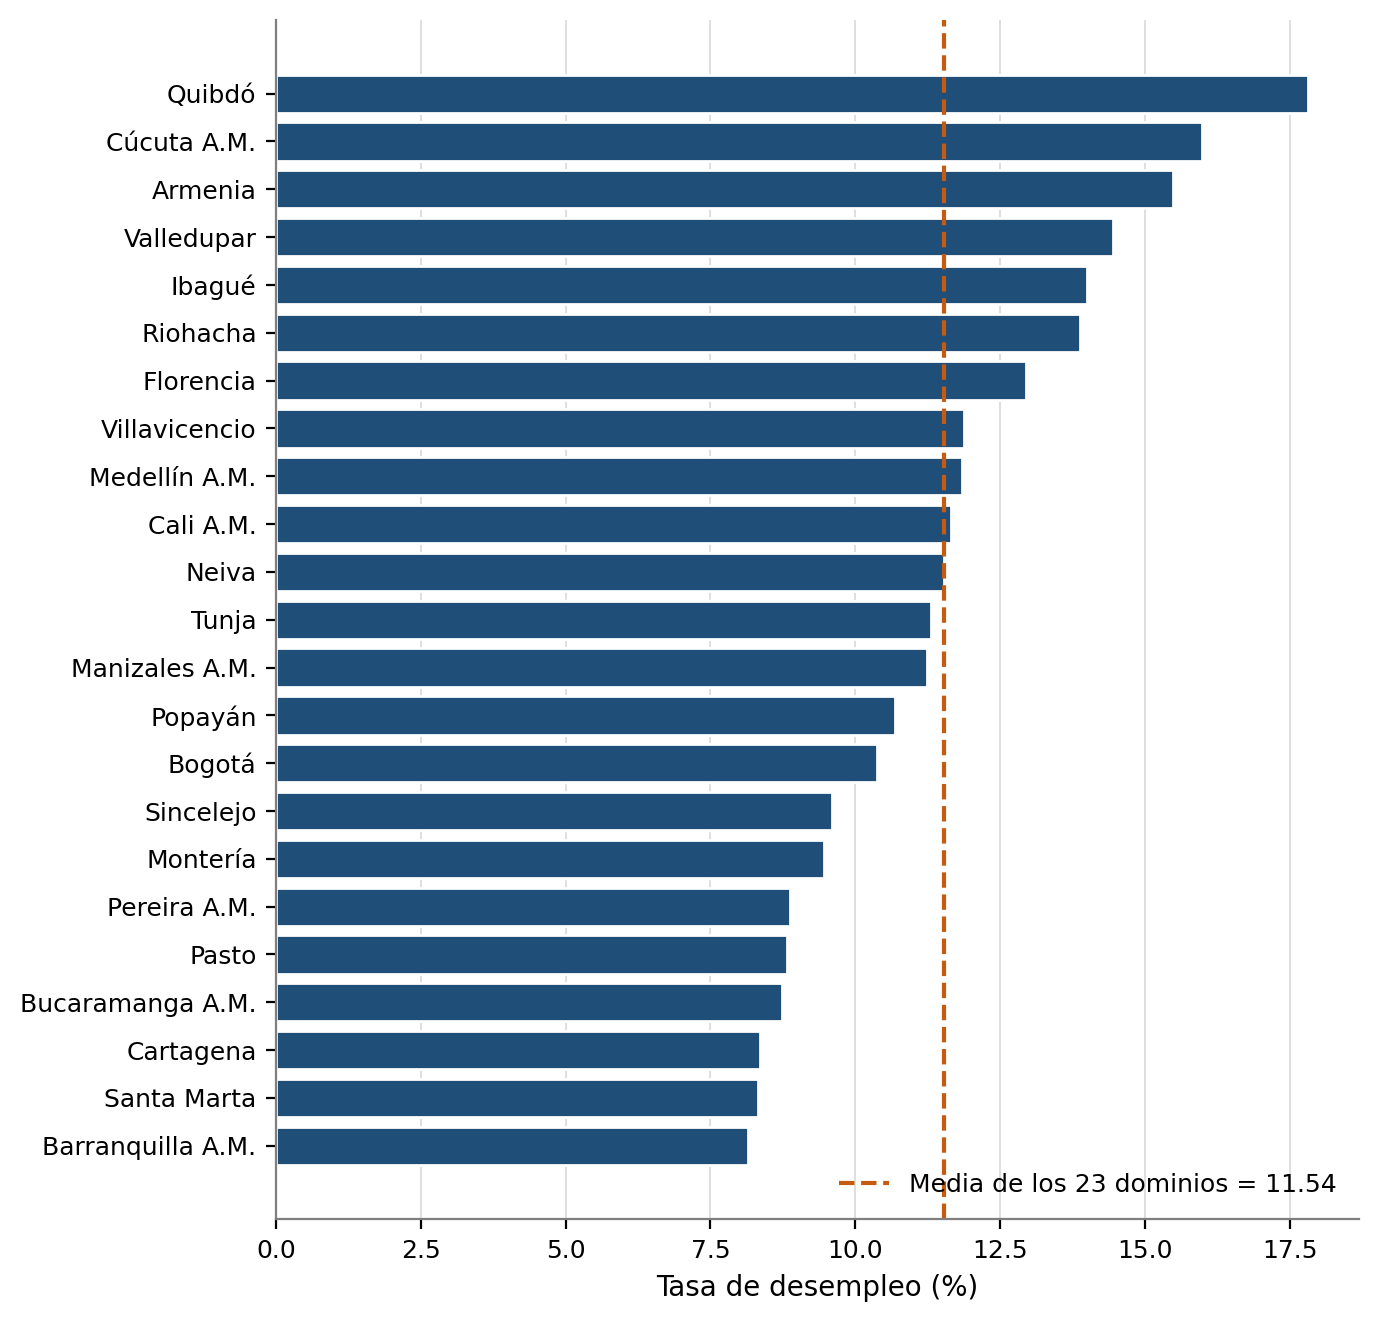
\includegraphics[width=0.9\linewidth]{img/desc_territorial_respuesta.png}
\caption{Tasa directa de los 23 dominios ordenada de mayor a menor, con su intervalo del 95~\%. Fuente: tablas del análisis descriptivo.}
\label{fig:app_territorial}
\end{figure}
\begin{figure}[!htbp]
\centering
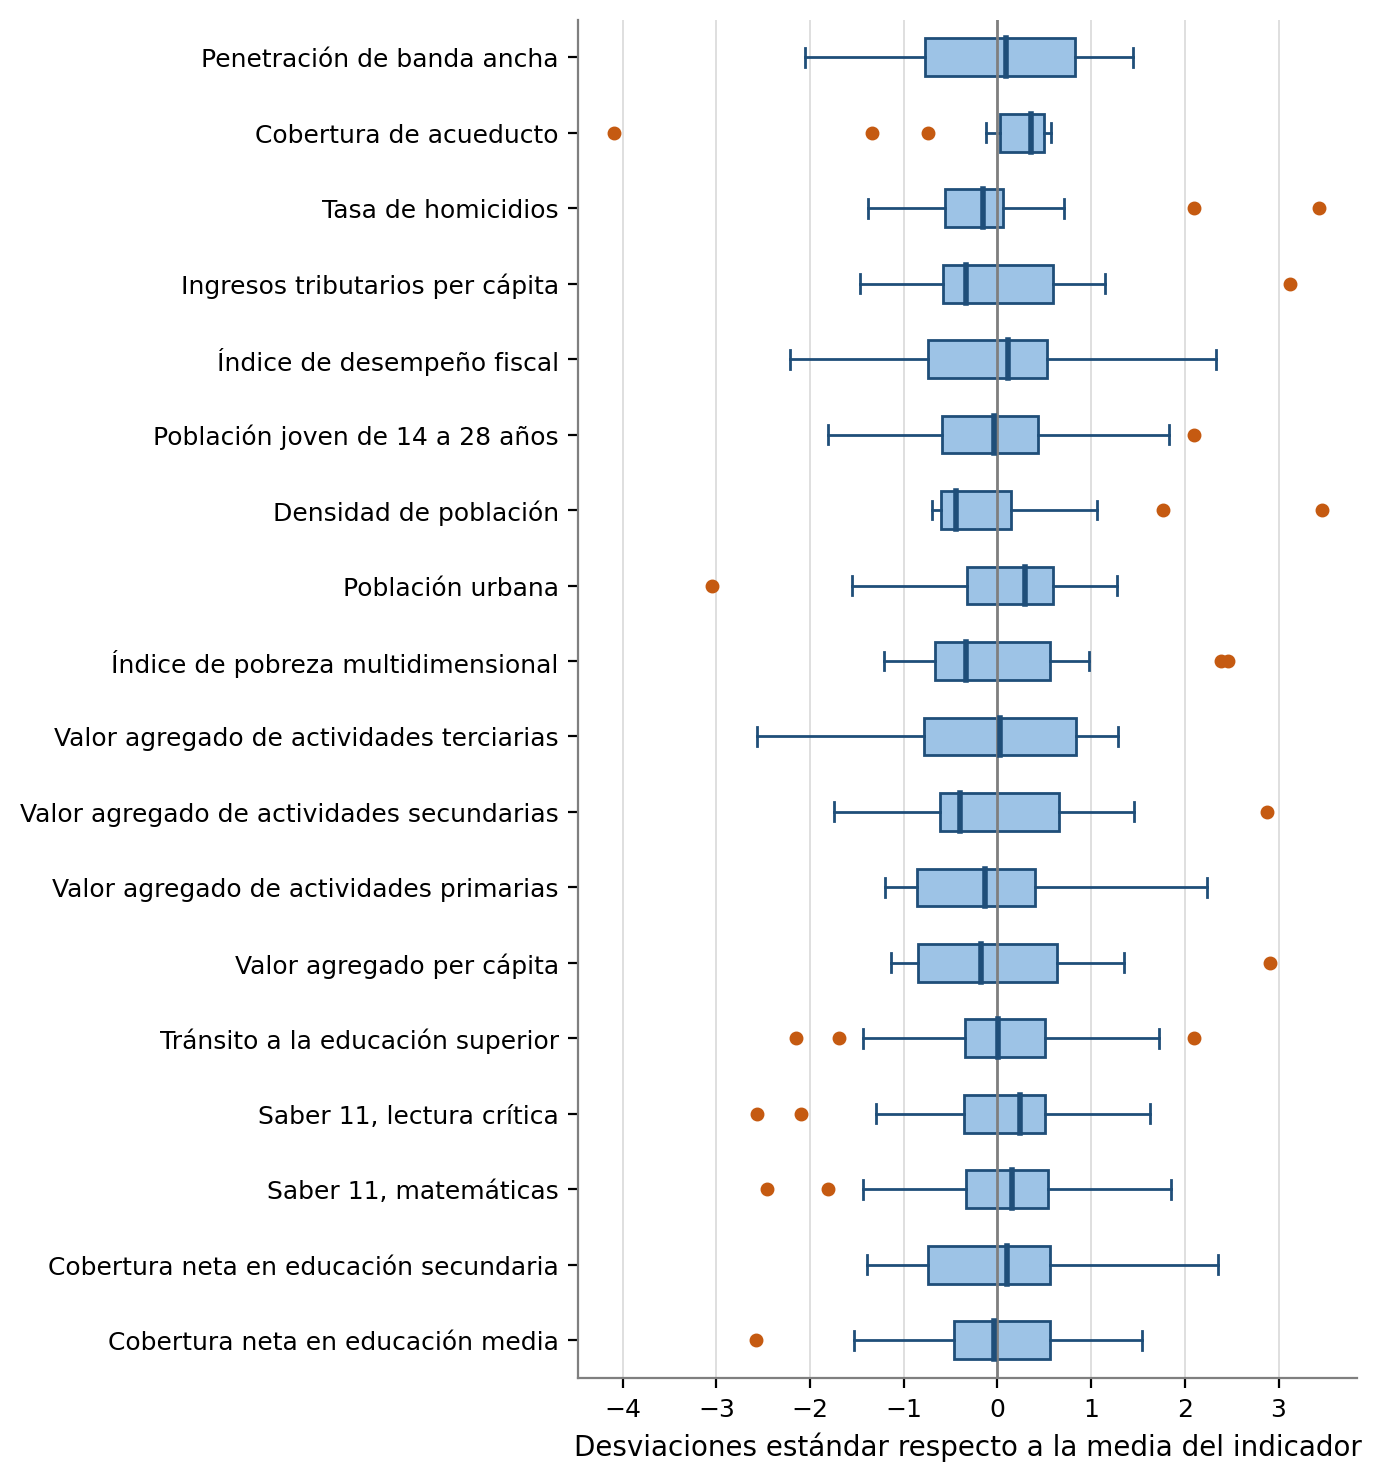
\includegraphics[width=0.9\linewidth]{img/desc_boxplots_candidatas.png}
\caption{Diagramas de caja de las 18 candidatas en escala estandarizada. Fuente: tablas del análisis descriptivo.}
\label{fig:app_boxplots}
\end{figure}
\begin{figure}[!htbp]
\centering
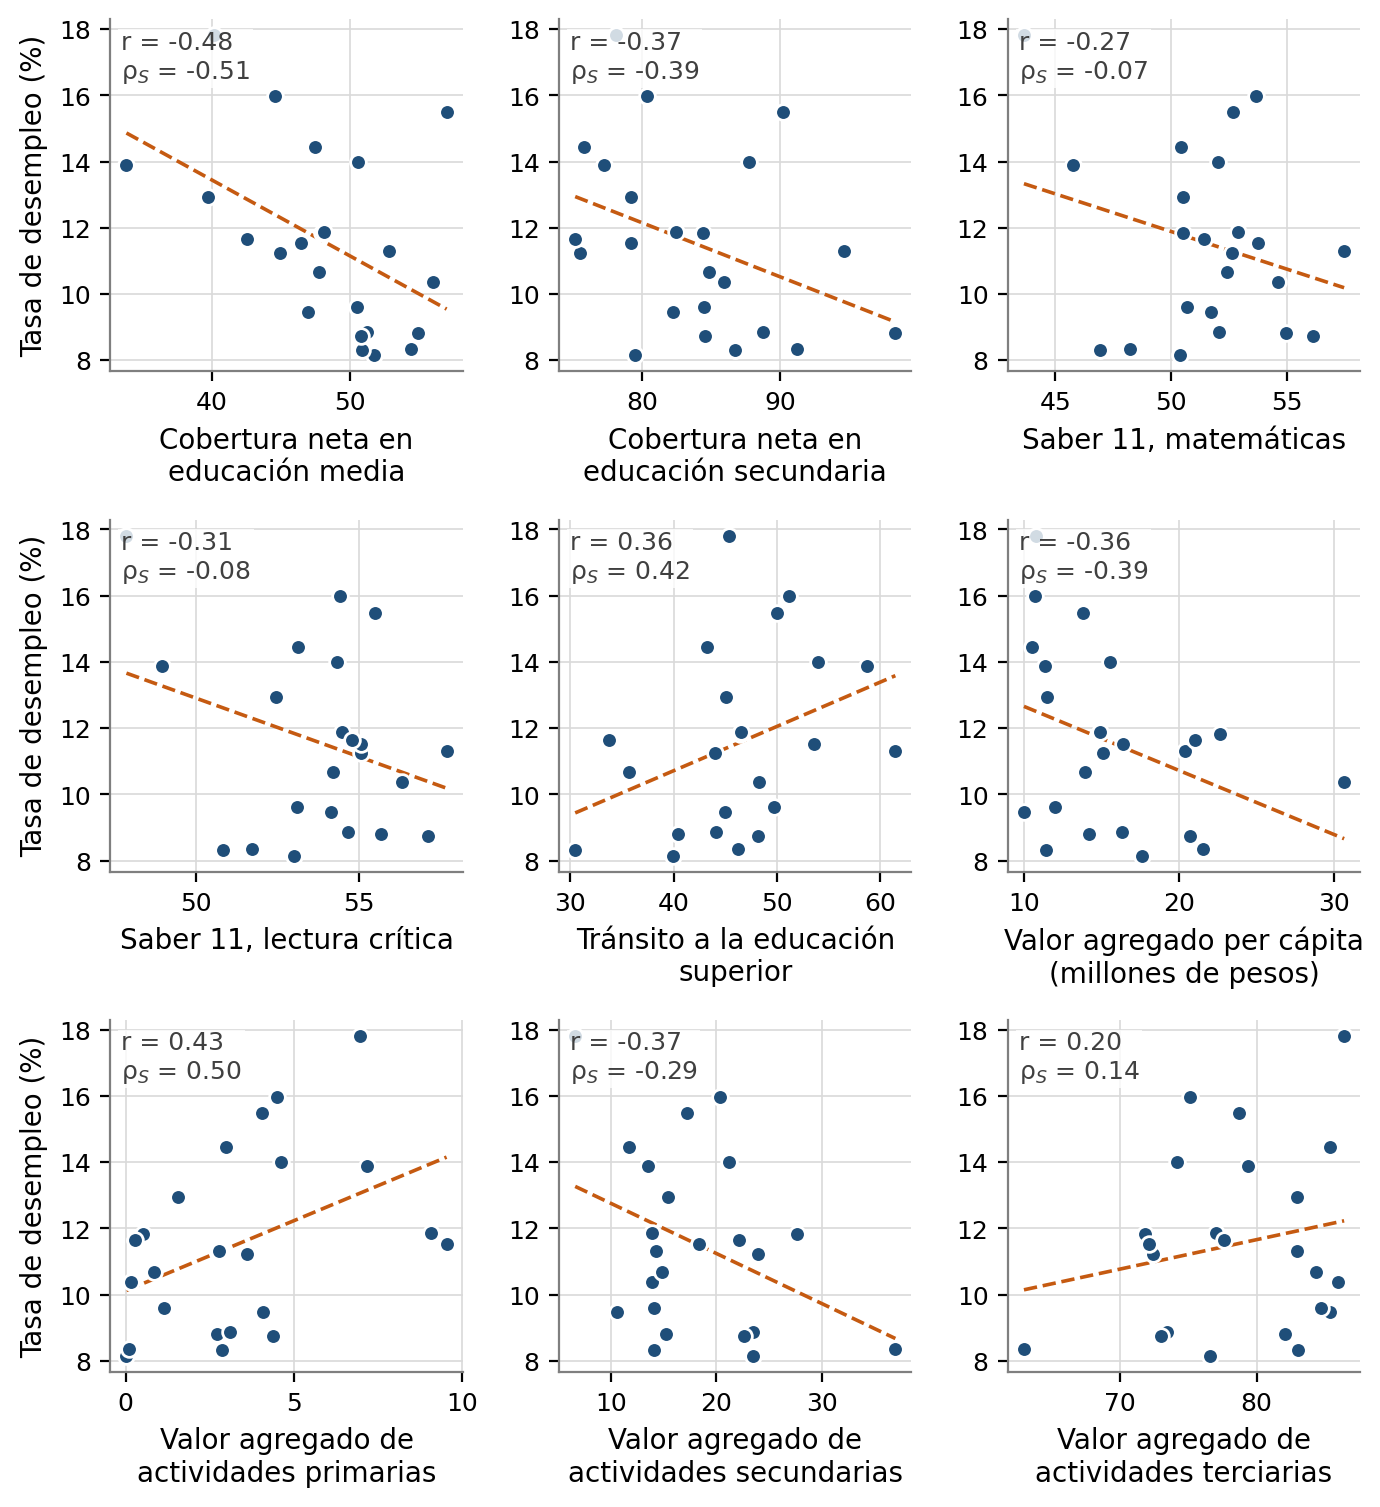
\includegraphics[width=0.9\linewidth]{img/desc_dispersion_candidatas_1.png}
\caption[Tasa directa frente a las candidatas (1 de 2)]{Tasa directa frente a las primeras nueve candidatas en los 23 dominios, con la recta de mínimos cuadrados como referencia. $r$: correlación de Pearson; $\rho_S$: correlación de Spearman. El valor agregado per cápita se expresa en millones de pesos. Fuente: tablas del análisis descriptivo.}
\label{fig:app_dispersion}
\end{figure}
\begin{figure}[!htbp]
\centering
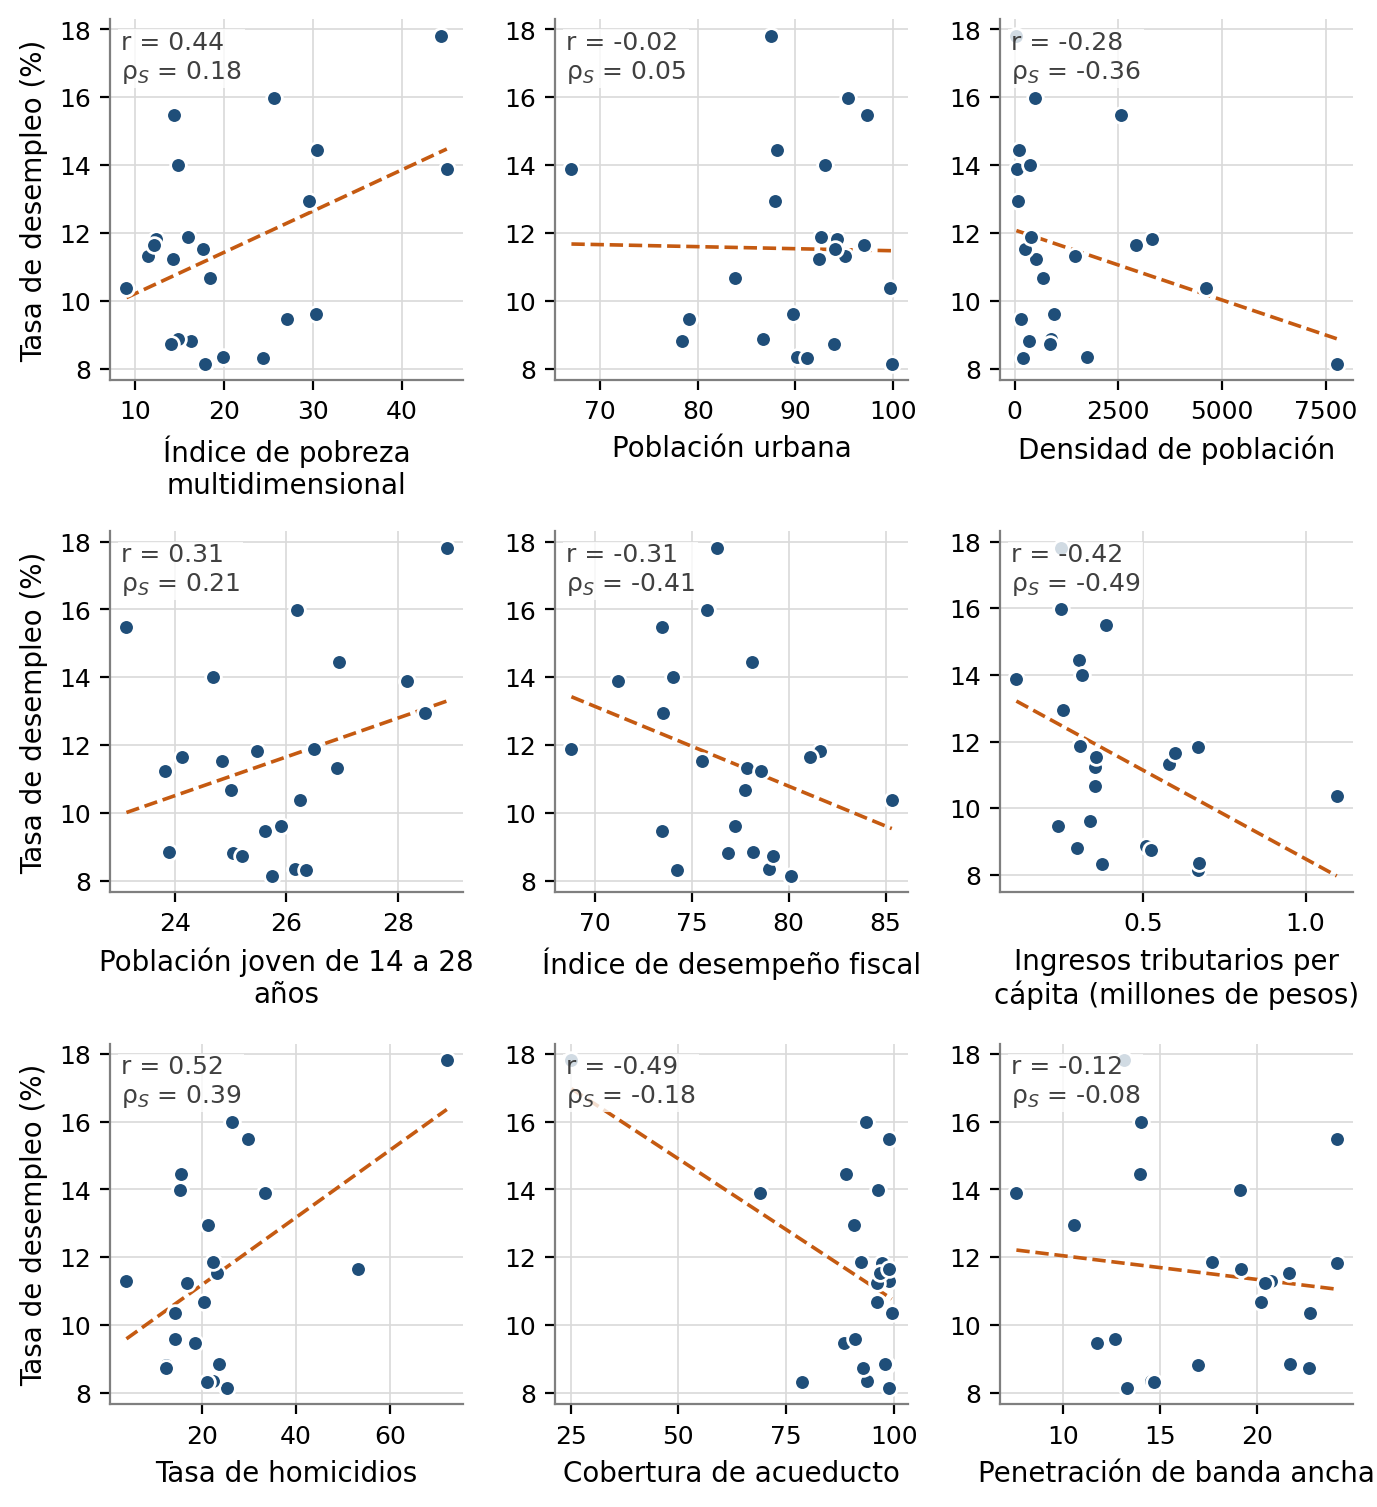
\includegraphics[width=0.9\linewidth]{img/desc_dispersion_candidatas_2.png}
\caption[Tasa directa frente a las candidatas (2 de 2)]{Tasa directa frente a las nueve candidatas restantes, con la misma lectura de la Figura~\ref{fig:app_dispersion}. Los ingresos tributarios per cápita se expresan en millones de pesos. Fuente: tablas del análisis descriptivo.}
\label{fig:app_dispersion_2}
\end{figure}
\begin{figure}[!htbp]
\centering
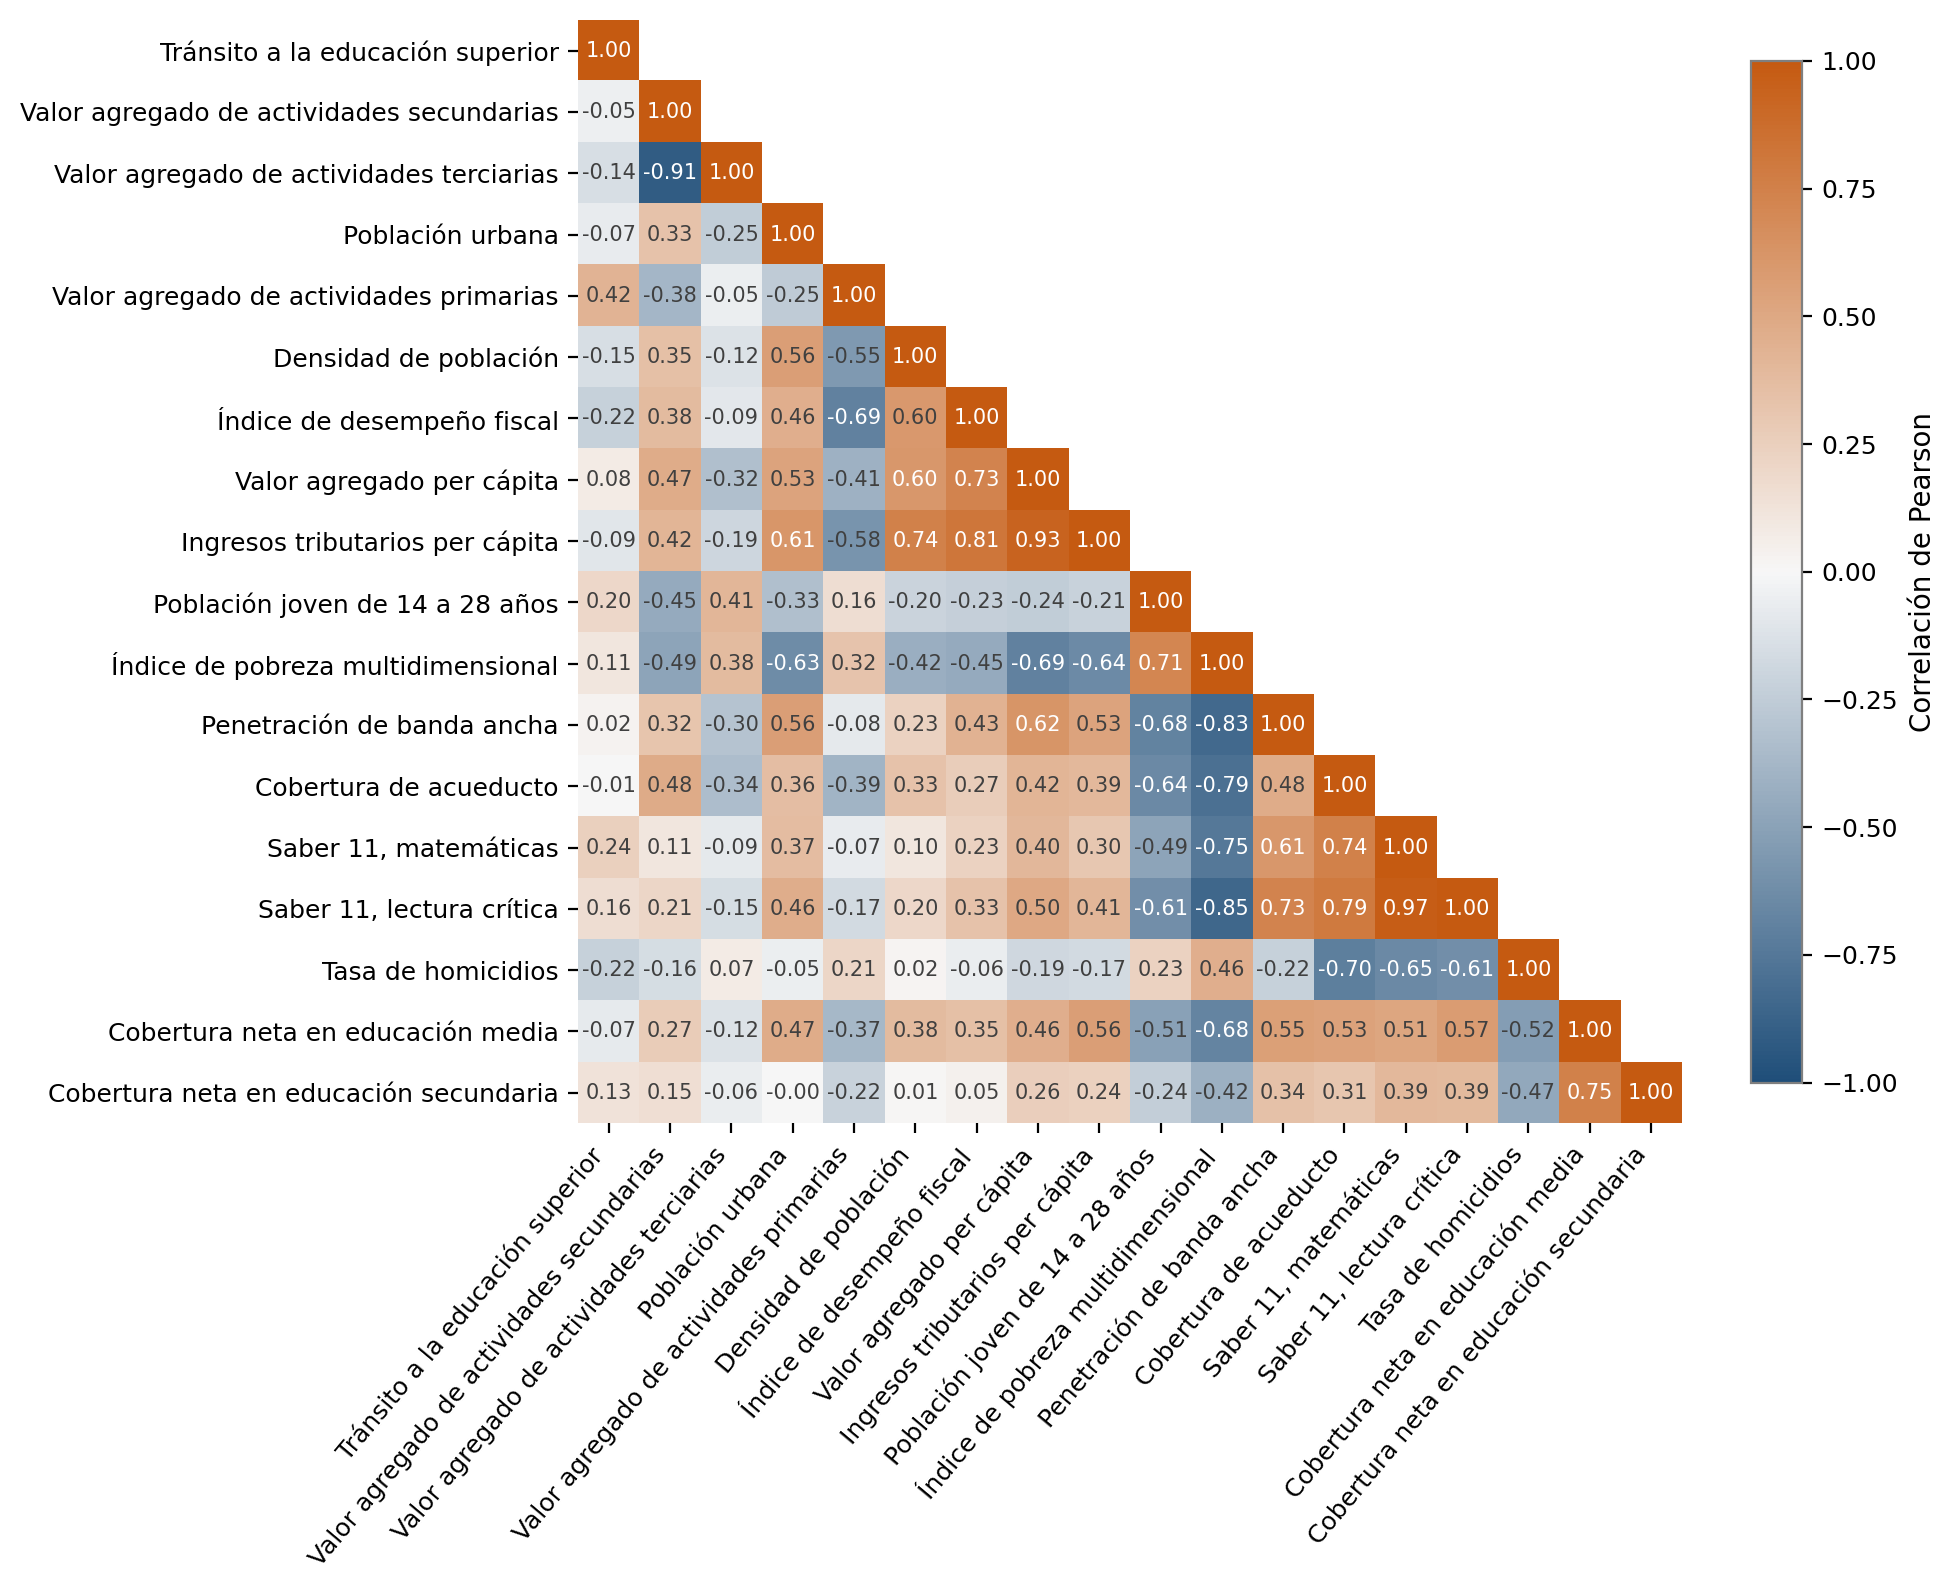
\includegraphics[width=0.9\linewidth]{img/desc_correlacion_candidatas.png}
\caption{Matriz de correlaciones de las candidatas, reordenada por agrupamiento. Fuente: tablas del análisis descriptivo.}
\label{fig:app_correlacion}
\end{figure}
%--------------------------------------------------------------------------------------
\anexo{Detalle de la selección de covariables}
\label{app:seleccion}

Esta sección presenta el Fay-Herriot univariado de cada candidata y los diagnósticos del conjunto elegido; la cita la Sección~\ref{sec:res_seleccion}.

La Tabla~\ref{tab:app_seleccion} ordena las 18 candidatas por el valor $p$ de su coeficiente. Solo tres tienen $q \le 0.10$ (tasa de homicidios, cobertura de acueducto y cobertura neta en educación media, las tres con $q = 0.079$), y Quibdó es el dominio que más mueve la correlación ponderada en ocho de las 18. Las dos covariables del conjunto elegido, tasa de homicidios y cobertura de acueducto, tienen una correlación de Pearson de $-0.70$ en los 23 dominios y un VIF de 1.984, por debajo del umbral de 5. La Figura~\ref{fig:app_residuos_parciales} muestra la relación de cada una con la tasa una vez descontado el aporte de la otra.

% D-40: la matriz de 2 por 2 (img/eda_correlacion_finales.png) se sustituyó por la frase anterior; r = -0.704 recalculado con _trabajo/calculos/datos/dominios.csv y VIF de la salida del cuaderno de selección.
{\footnotesize\setlength{\tabcolsep}{3pt}
\begin{longtable}{p{2.4cm} r p{2.3cm} r r r p{1.9cm} r}
\caption[Fay-Herriot univariado de cada candidata]{Fay-Herriot univariado de cada candidata, ajustado por REML (máxima verosimilitud restringida) y GLS (mínimos cuadrados generalizados). IC: intervalo de confianza de Wald; $q$: valor ajustado por Benjamini-Hochberg; Cook: distancia máxima; Dominio: el que más cambia $r_w$ al retirarlo; $\Delta r_w$: ese cambio; A.M.: área metropolitana. Los coeficientes están en la unidad de cada covariable, salvo el valor agregado per cápita y los ingresos tributarios per cápita (por millón de pesos) y la densidad de población (por cada 1,000 habitantes por km$^2$).}
\label{tab:app_seleccion} \\
\toprule
Covariable & $\hat{\beta}_1$ & IC 95~\% & $p$ & $q$ & Cook & Dominio & $\Delta r_w$ \\
\midrule
\endfirsthead
\multicolumn{8}{l}{\tablename~\thetable{}, continuación} \\
\toprule
Covariable & $\hat{\beta}_1$ & IC 95~\% & $p$ & $q$ & Cook & Dominio & $\Delta r_w$ \\
\midrule
\endhead
\bottomrule
\endlastfoot
Tasa de homicidios & 0.099 & [0.029, 0.170] & 0.006 & 0.079 & 0.601 & Quibdó & 0.270 \\
Cobertura de acueducto & $-0.083$ & [$-0.147$, $-0.019$] & 0.011 & 0.079 & 1.297 & Quibdó & 0.388 \\
Cobertura neta en educación media & $-0.229$ & [$-0.410$, $-0.048$] & 0.013 & 0.079 & 0.625 & Armenia & 0.177 \\
Índice de pobreza multidimensional & 0.121 & [0.015, 0.226] & 0.025 & 0.101 & 0.577 & Quibdó & 0.198 \\
Valor agregado de actividades primarias & 0.422 & [0.045, 0.798] & 0.028 & 0.101 & 0.278 & Quibdó & 0.082 \\
Ingresos tributarios per cápita & $-5.281$ & [$-10.155$, $-0.407$] & 0.034 & 0.101 & 0.845 & Bogotá & 0.069 \\
Cobertura neta en educación secundaria & $-0.163$ & [$-0.336$, 0.011] & 0.066 & 0.135 & 0.212 & Armenia & 0.109 \\
Valor agregado de actividades secundarias & $-0.150$ & [$-0.314$, 0.013] & 0.072 & 0.135 & 0.411 & Quibdó & 0.146 \\
Valor agregado per cápita & $-0.192$ & [$-0.403$, 0.019] & 0.074 & 0.135 & 0.286 & Santa Marta & 0.070 \\
Tránsito a la educación superior & 0.134 & [$-0.014$, 0.281] & 0.075 & 0.135 & 0.163 & Santa Marta & 0.080 \\
Índice de desempeño fiscal & $-0.234$ & [$-0.536$, 0.067] & 0.128 & 0.202 & 0.130 & Santa Marta & 0.058 \\
Población joven de 14 a 28 años & 0.567 & [$-0.183$, 1.318] & 0.138 & 0.202 & 0.637 & Quibdó & 0.206 \\
Saber 11, lectura crítica & $-0.352$ & [$-0.826$, 0.122] & 0.146 & 0.202 & 0.962 & Quibdó & 0.271 \\
Densidad de población & $-0.410$ & [$-1.007$, 0.186] & 0.177 & 0.228 & 0.172 & Barranquilla A.M. & 0.162 \\
Saber 11, matemáticas & $-0.224$ & [$-0.572$, 0.123] & 0.206 & 0.247 & 0.953 & Quibdó & 0.270 \\
Valor agregado de actividades terciarias & 0.088 & [$-0.098$, 0.274] & 0.353 & 0.398 & 0.315 & Cartagena & 0.130 \\
Penetración de banda ancha & $-0.069$ & [$-0.312$, 0.175] & 0.581 & 0.615 & 0.241 & Armenia & 0.125 \\
Población urbana & $-0.006$ & [$-0.159$, 0.146] & 0.938 & 0.938 & 0.524 & Riohacha & 0.166 \\
\end{longtable}
}
\begin{figure}[!htbp]
\centering
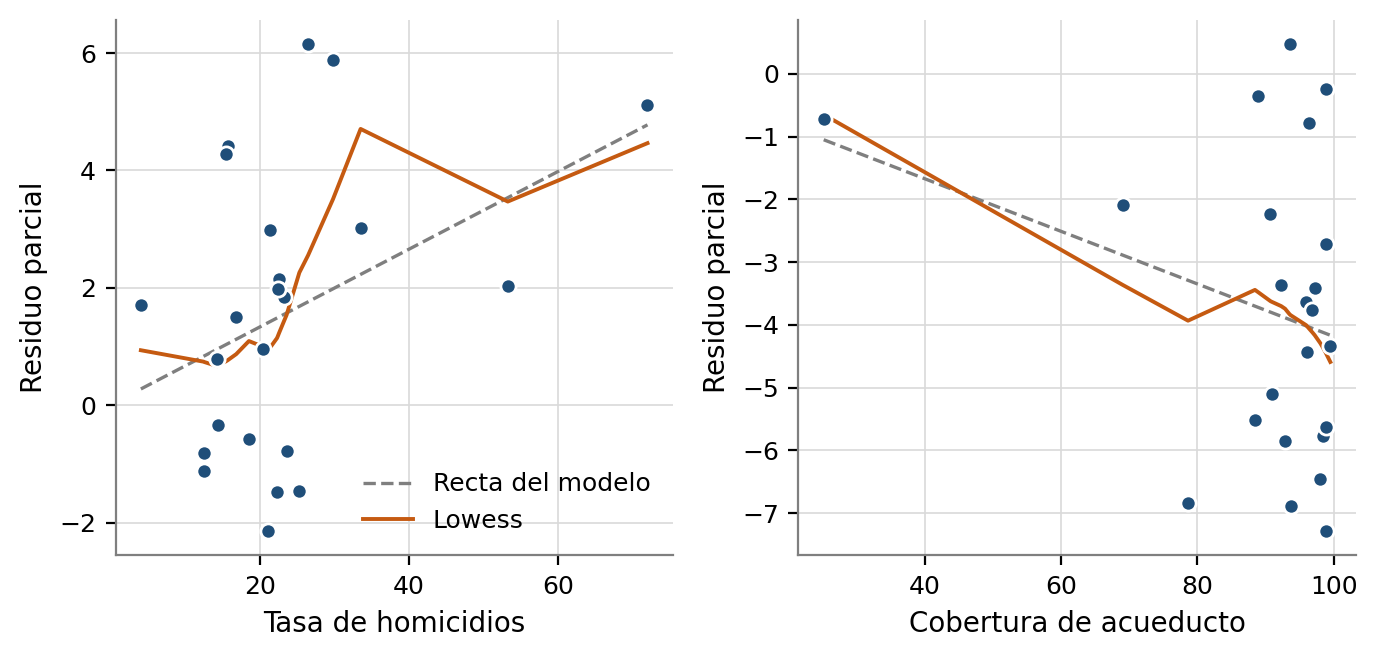
\includegraphics[width=0.9\linewidth]{img/eda_residuos_parciales.png}
\caption{Residuos parciales de las covariables seleccionadas en el Fay-Herriot con ambas. Fuente: tabla de verificación de la selección.}
\label{fig:app_residuos_parciales}
\end{figure}
%--------------------------------------------------------------------------------------
\anexo{Especificaciones del Fay-Herriot clásico}
\label{app:especificaciones}

Esta sección presenta los coeficientes y los diagnósticos de las cuatro especificaciones candidatas; la citan las Secciones~\ref{sec:res_fh_clasico} y~\ref{sec:res_supuestos}.

La Tabla~\ref{tab:app_ec_coeficientes} muestra que en EC1, con las dos covariables, ninguna tiene $p < 0.05$, mientras que en EC2 y EC3, con una covariable cada una, las dos lo cumplen. En la Tabla~\ref{tab:app_ec_diagnosticos} el valor $p$ de Shapiro-Wilk supera 0.10 en las cuatro especificaciones y EC2 tiene la mayor distancia de Cook (1.297). Las Figuras~\ref{fig:app_ec3}, \ref{fig:app_ec1}, \ref{fig:app_ec2} y~\ref{fig:app_ec0} muestran, para cada especificación, la contracción del EBLUP y la distribución de los residuos estandarizados, y la Figura~\ref{fig:app_cook} identifica los dominios que más pesan en el ajuste del benchmark.

\begin{table}[!htbp]
\centering
\small
\caption[Coeficientes de las especificaciones candidatas]{Coeficientes de las cuatro especificaciones candidatas. EE: error estándar. Fuente: salida del cuaderno del Fay-Herriot clásico.}
\label{tab:app_ec_coeficientes}
\begin{tabular}{l l r r r}
\toprule
Especificación & Parámetro & $\hat{\beta}$ & EE & $p$ \\
\midrule
EC1 & Intercepto & 13.758 & 4.997 & 0.006 \\
EC1 & Tasa de homicidios & 0.066 & 0.051 & 0.190 \\
EC1 & Cobertura de acueducto & $-0.042$ & 0.045 & 0.351 \\
EC2 & Intercepto & 19.053 & 2.994 & $<0.001$ \\
EC2 & Cobertura de acueducto & $-0.083$ & 0.033 & 0.011 \\
EC3 & Intercepto & 9.191 & 0.979 & $<0.001$ \\
EC3 & Tasa de homicidios & 0.099 & 0.036 & 0.006 \\
EC0 & Intercepto & 11.527 & 0.563 & $<0.001$ \\
\bottomrule
\end{tabular}
\end{table}
\begin{table}[!htbp]
\centering
\small
\caption[Diagnósticos de las especificaciones candidatas]{Diagnósticos de las especificaciones. DE resid.: desviación de los residuos estandarizados; SW: Shapiro-Wilk; $\psi/{\rm ECM}$: razón media entre la varianza directa y el error cuadrático medio (ECM) del EBLUP (mejor predictor lineal insesgado empírico); Influyentes: dominios con Cook $> 4/n$.}
\label{tab:app_ec_diagnosticos}
\begin{tabular}{l r r r r r r r}
\toprule
Especificación & $R^2$ & DE resid. & $p$ SW & $\bar{\gamma}$ & $\psi/{\rm ECM}$ & Cook & Influyentes \\
\midrule
EC1 & 0.299 & 0.954 & 0.391 & 0.984 & 1.011 & 0.526 & 2 \\
EC2 & 0.239 & 0.978 & 0.317 & 0.985 & 1.011 & 1.297 & 1 \\
EC3 & 0.269 & 0.977 & 0.357 & 0.984 & 1.012 & 0.601 & 2 \\
EC0 & 0.000 & 1.002 & 0.139 & 0.988 & 1.010 & 0.250 & 1 \\
\bottomrule
\end{tabular}
\end{table}
\begin{figure}[!htbp]
\centering
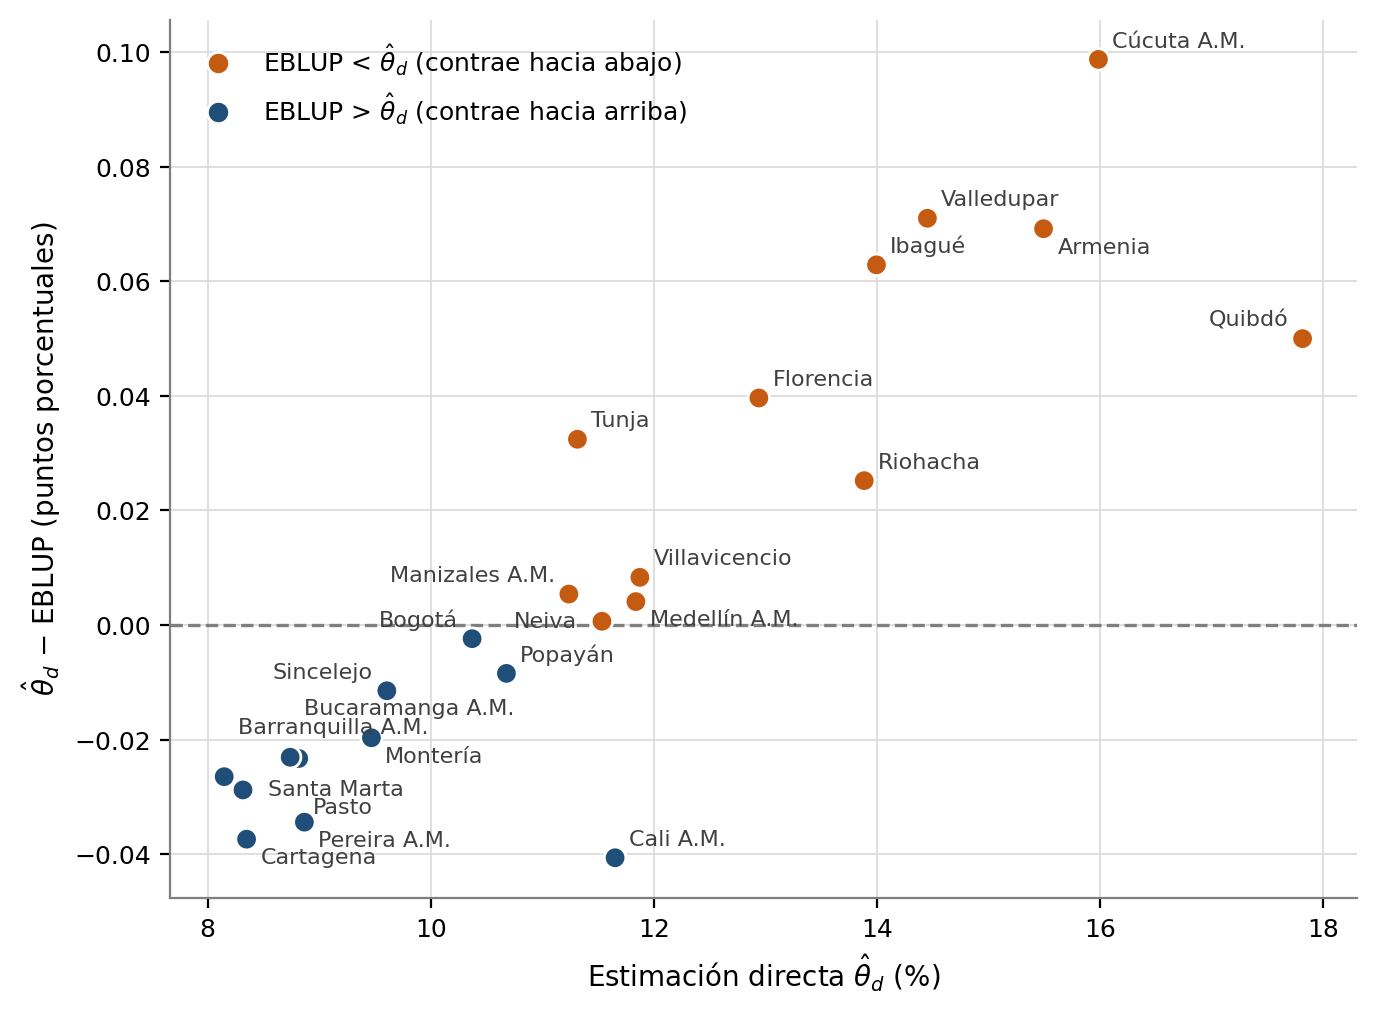
\includegraphics[width=0.48\linewidth]{img/fh_ec3_suavizador.png}
\hfill
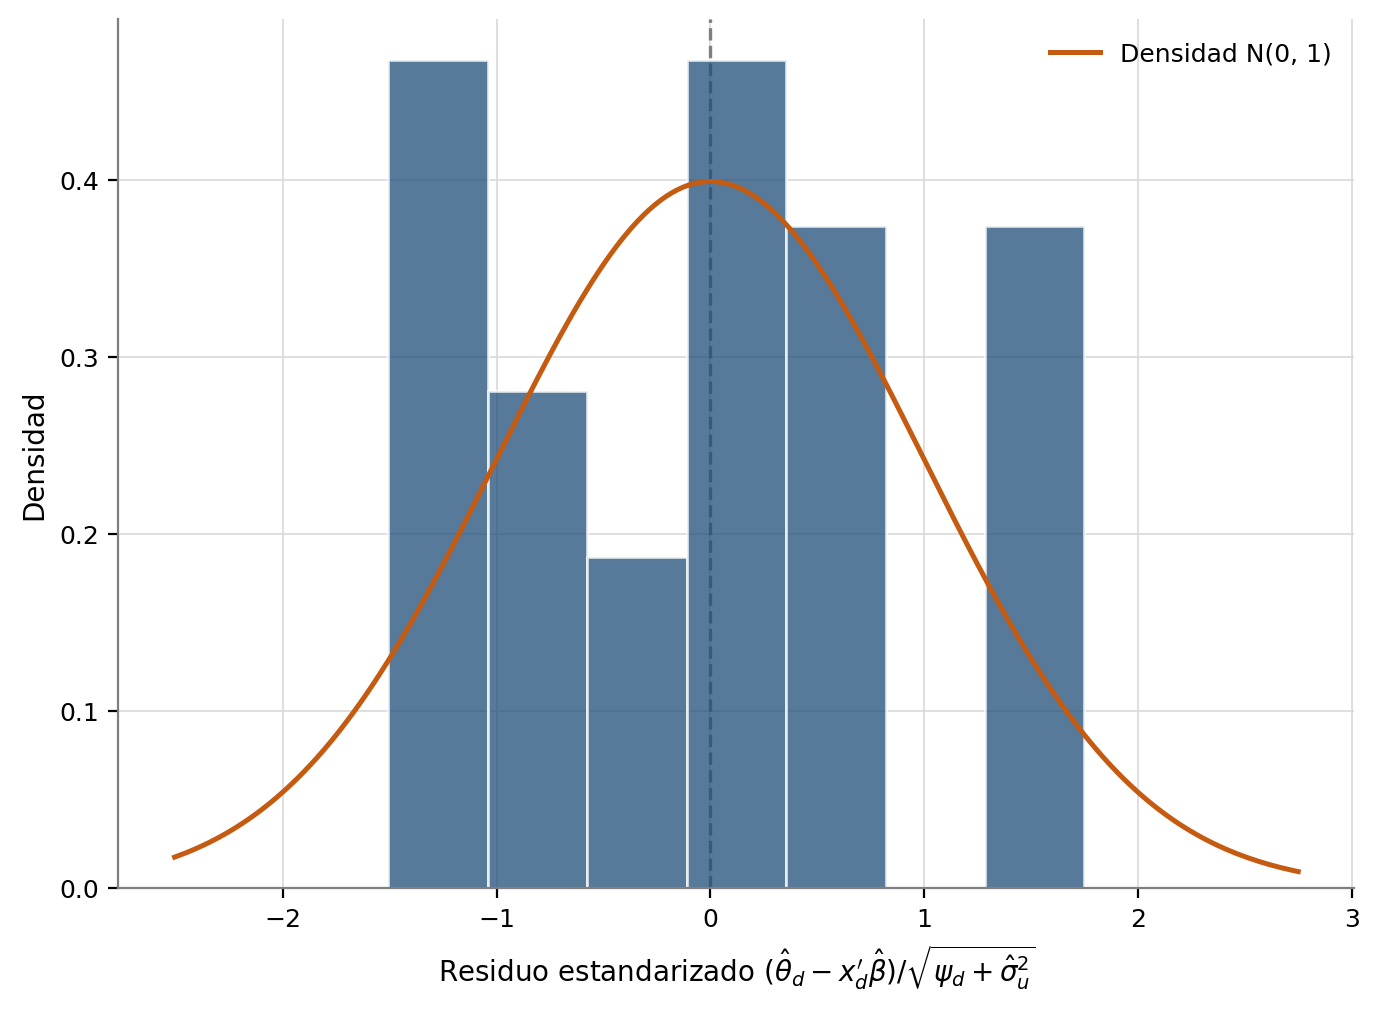
\includegraphics[width=0.48\linewidth]{img/fh_ec3_histograma.png}
\caption{Especificación EC3 (benchmark): a la izquierda, residuo del EBLUP frente a la tasa directa (contracción); a la derecha, histograma de los residuos estandarizados. Fuente: cuaderno del Fay-Herriot clásico.}
\label{fig:app_ec3}
\end{figure}
\begin{figure}[!htbp]
\centering
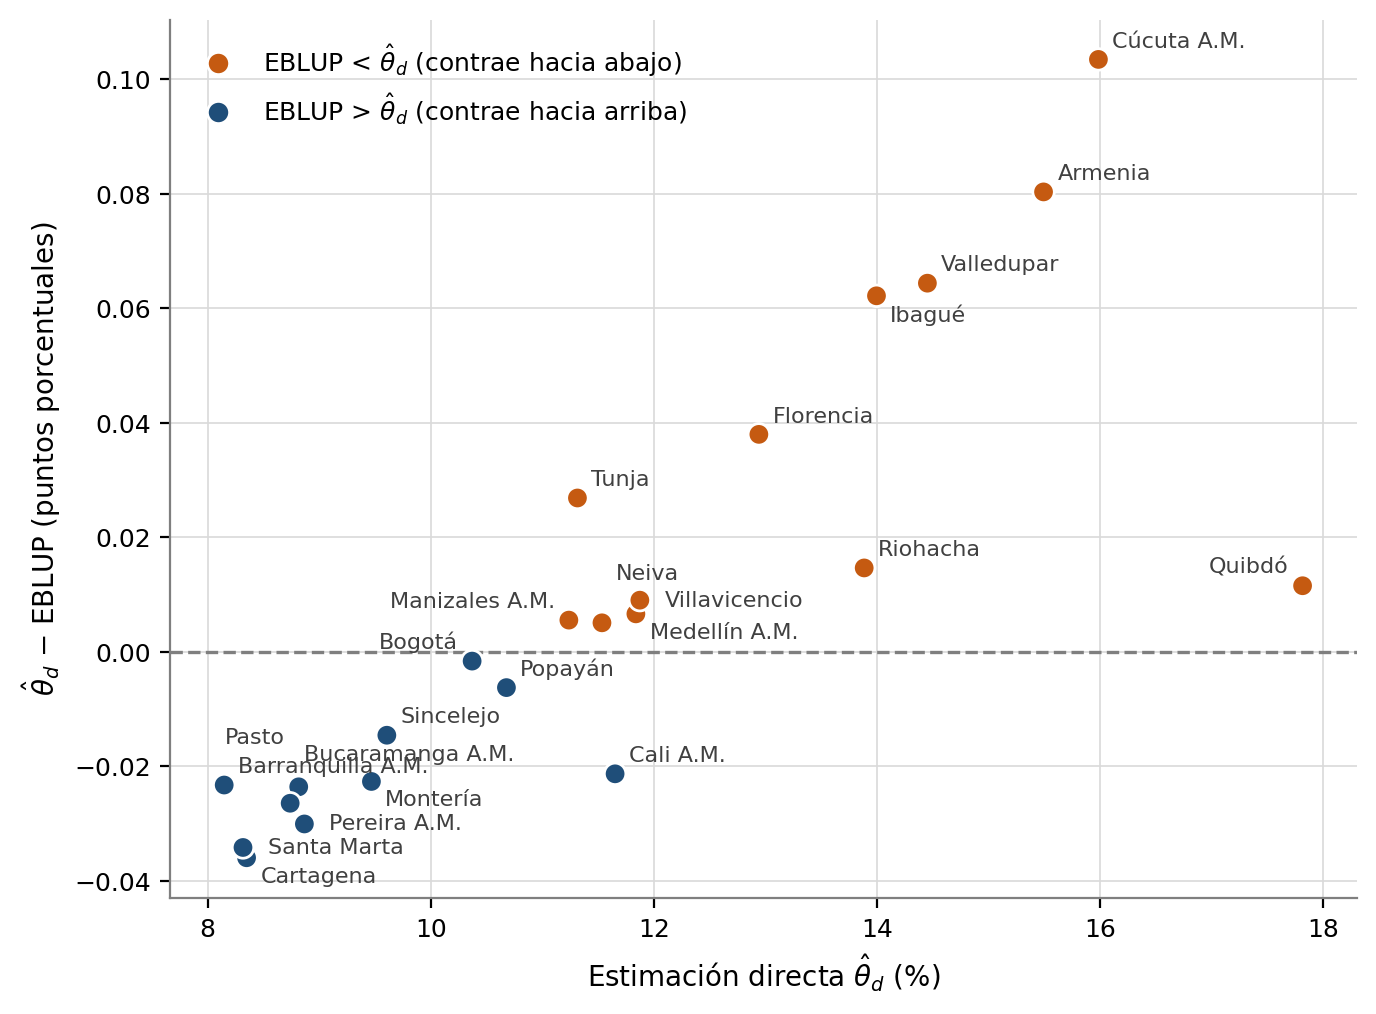
\includegraphics[width=0.48\linewidth]{img/fh_ec1_suavizador.png}
\hfill
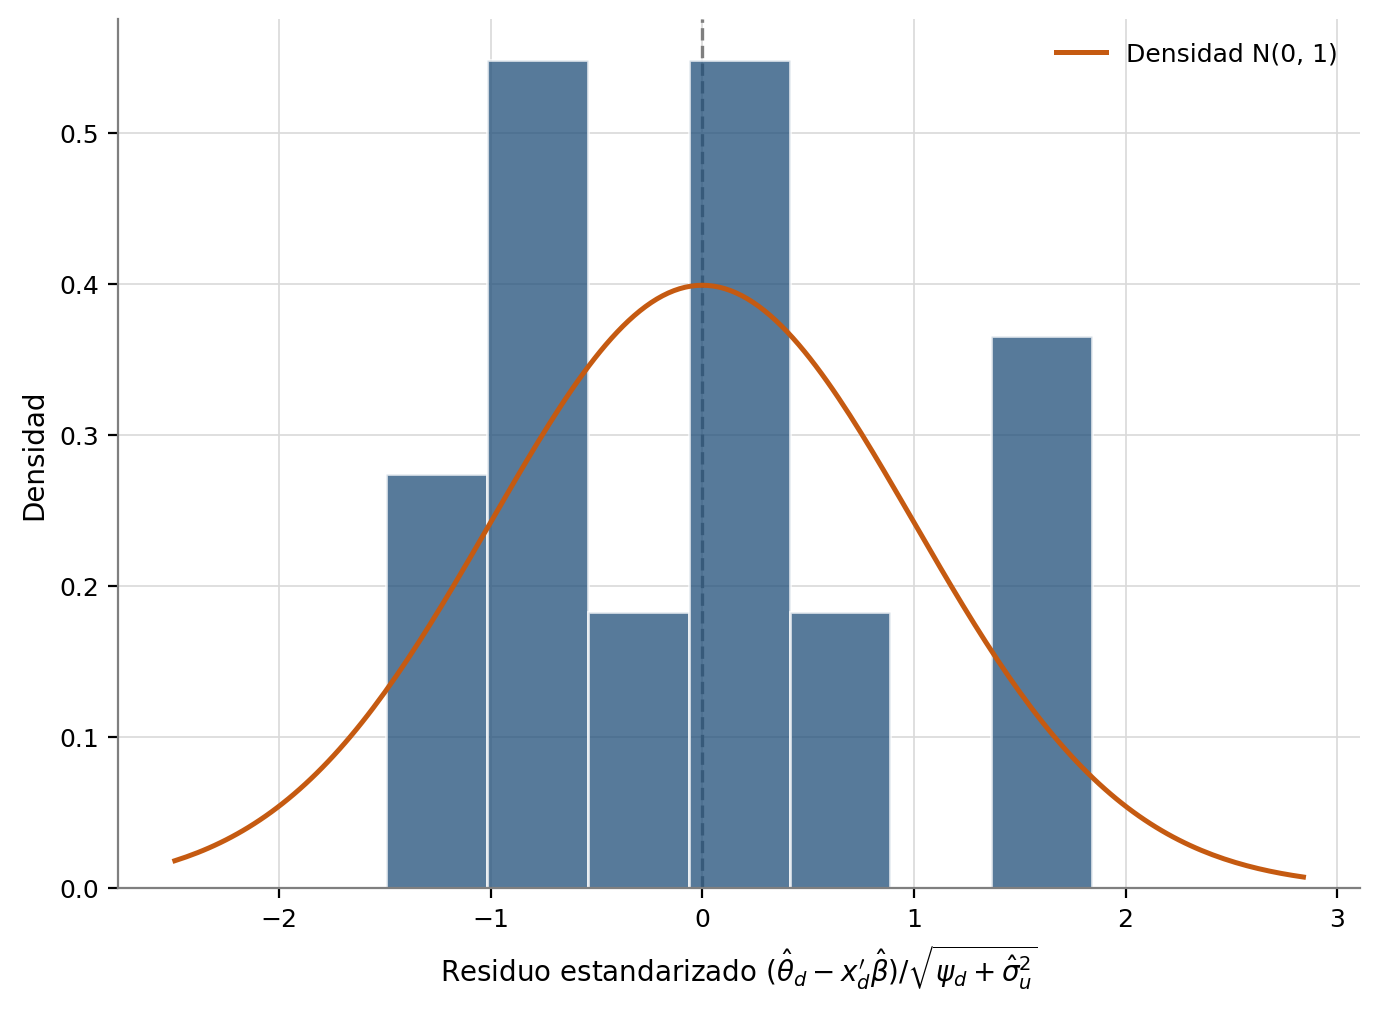
\includegraphics[width=0.48\linewidth]{img/fh_ec1_histograma.png}
\caption{Especificación EC1: a la izquierda, residuo del EBLUP frente a la tasa directa (contracción); a la derecha, histograma de los residuos estandarizados. Fuente: cuaderno del Fay-Herriot clásico.}
\label{fig:app_ec1}
\end{figure}
\begin{figure}[!htbp]
\centering
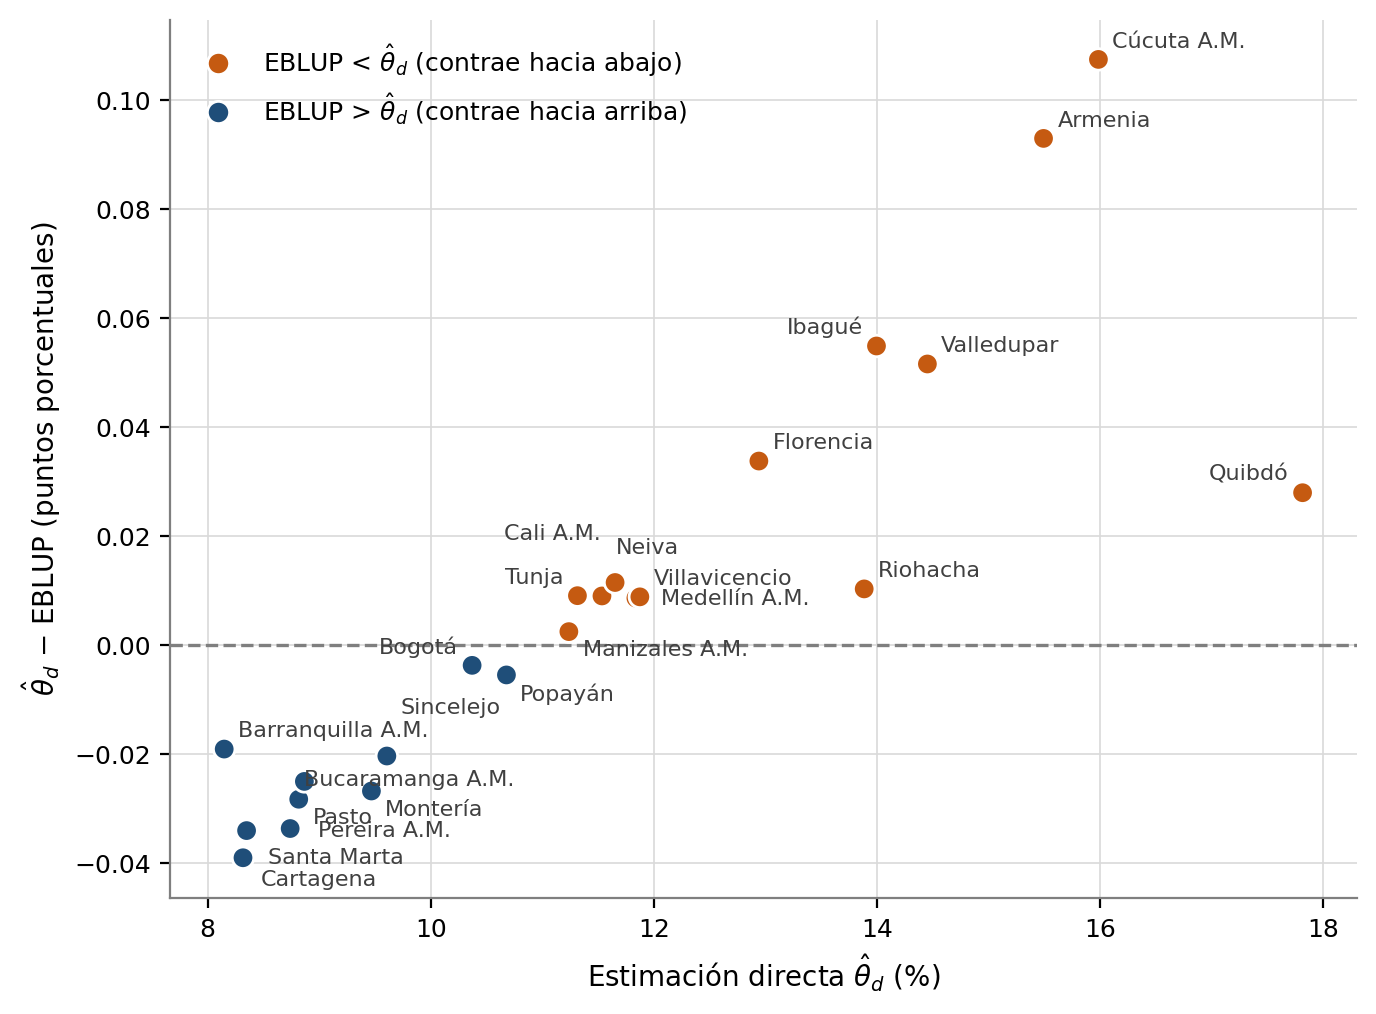
\includegraphics[width=0.48\linewidth]{img/fh_ec2_suavizador.png}
\hfill
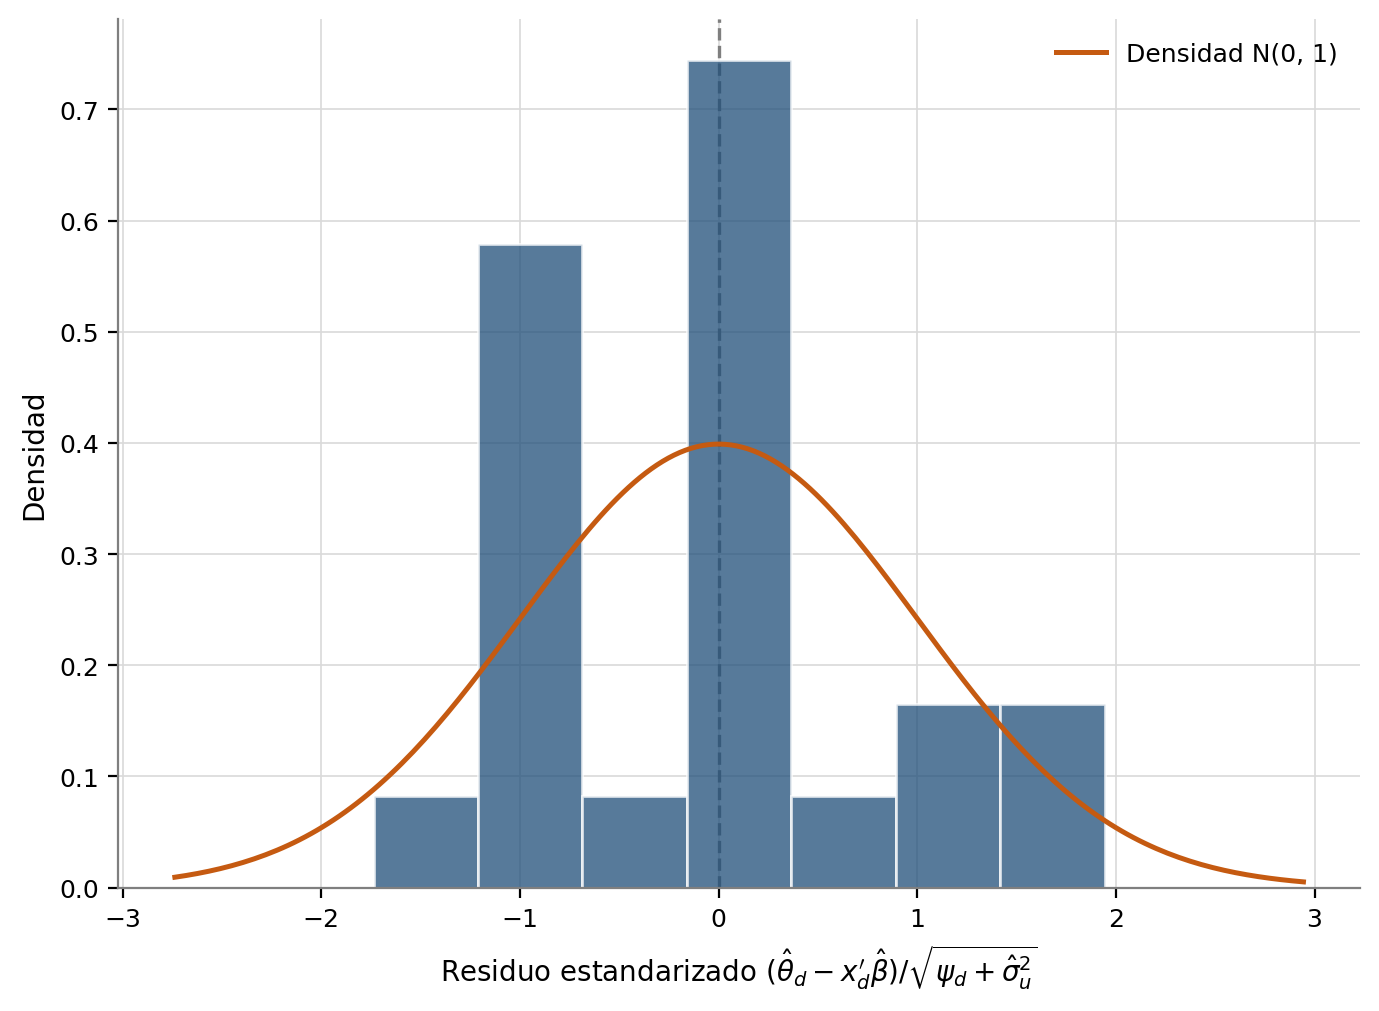
\includegraphics[width=0.48\linewidth]{img/fh_ec2_histograma.png}
\caption{Especificación EC2: a la izquierda, residuo del EBLUP frente a la tasa directa (contracción); a la derecha, histograma de los residuos estandarizados. Fuente: cuaderno del Fay-Herriot clásico.}
\label{fig:app_ec2}
\end{figure}
\begin{figure}[!htbp]
\centering
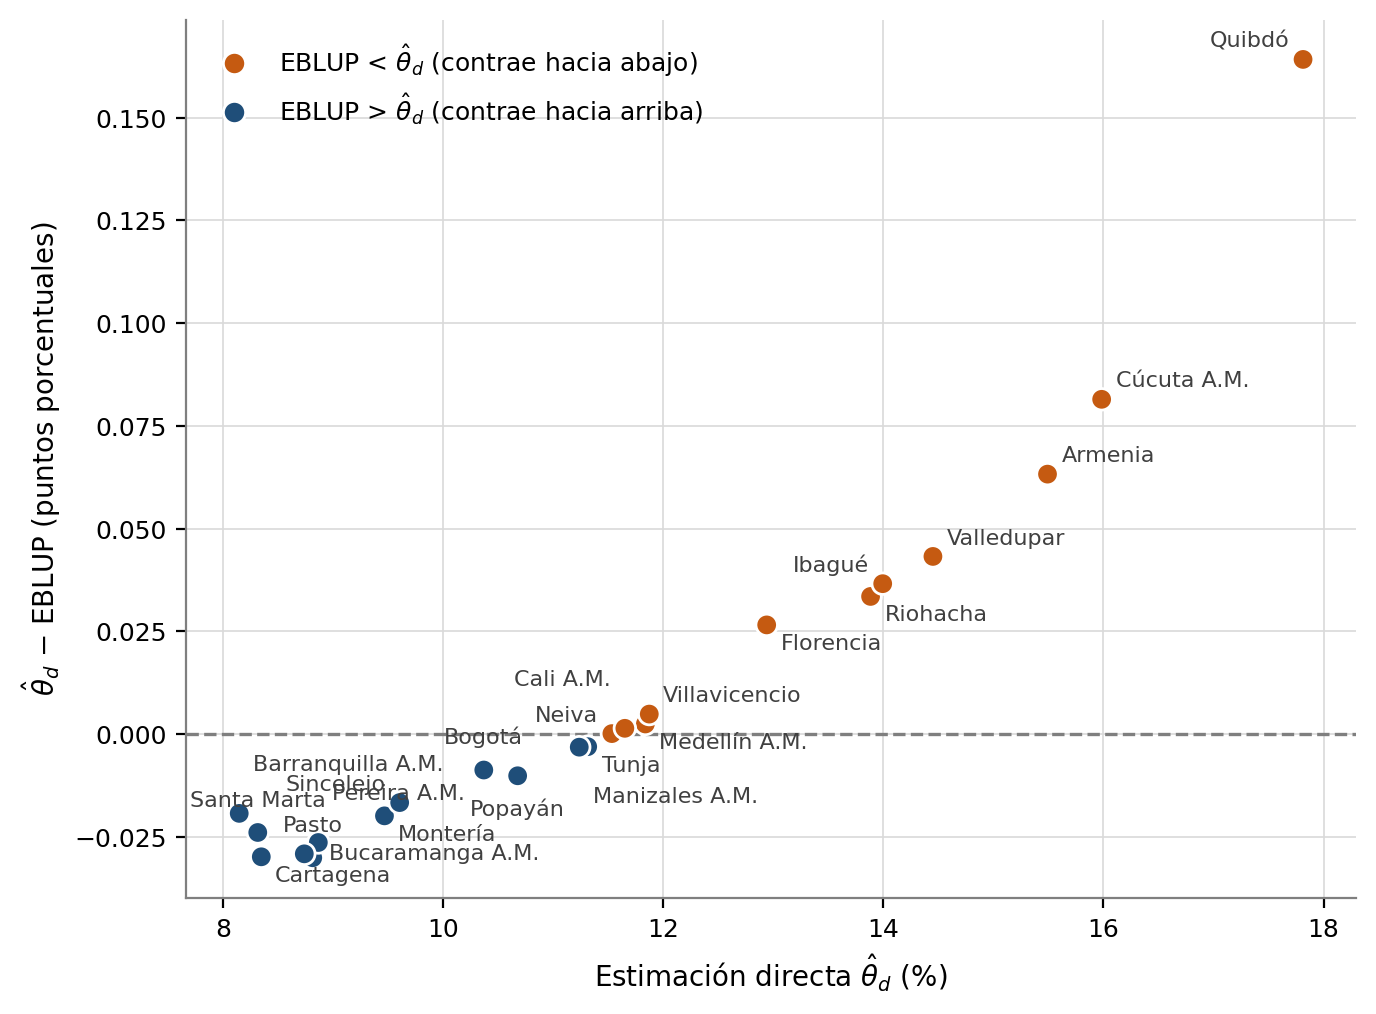
\includegraphics[width=0.48\linewidth]{img/fh_ec0_suavizador.png}
\hfill
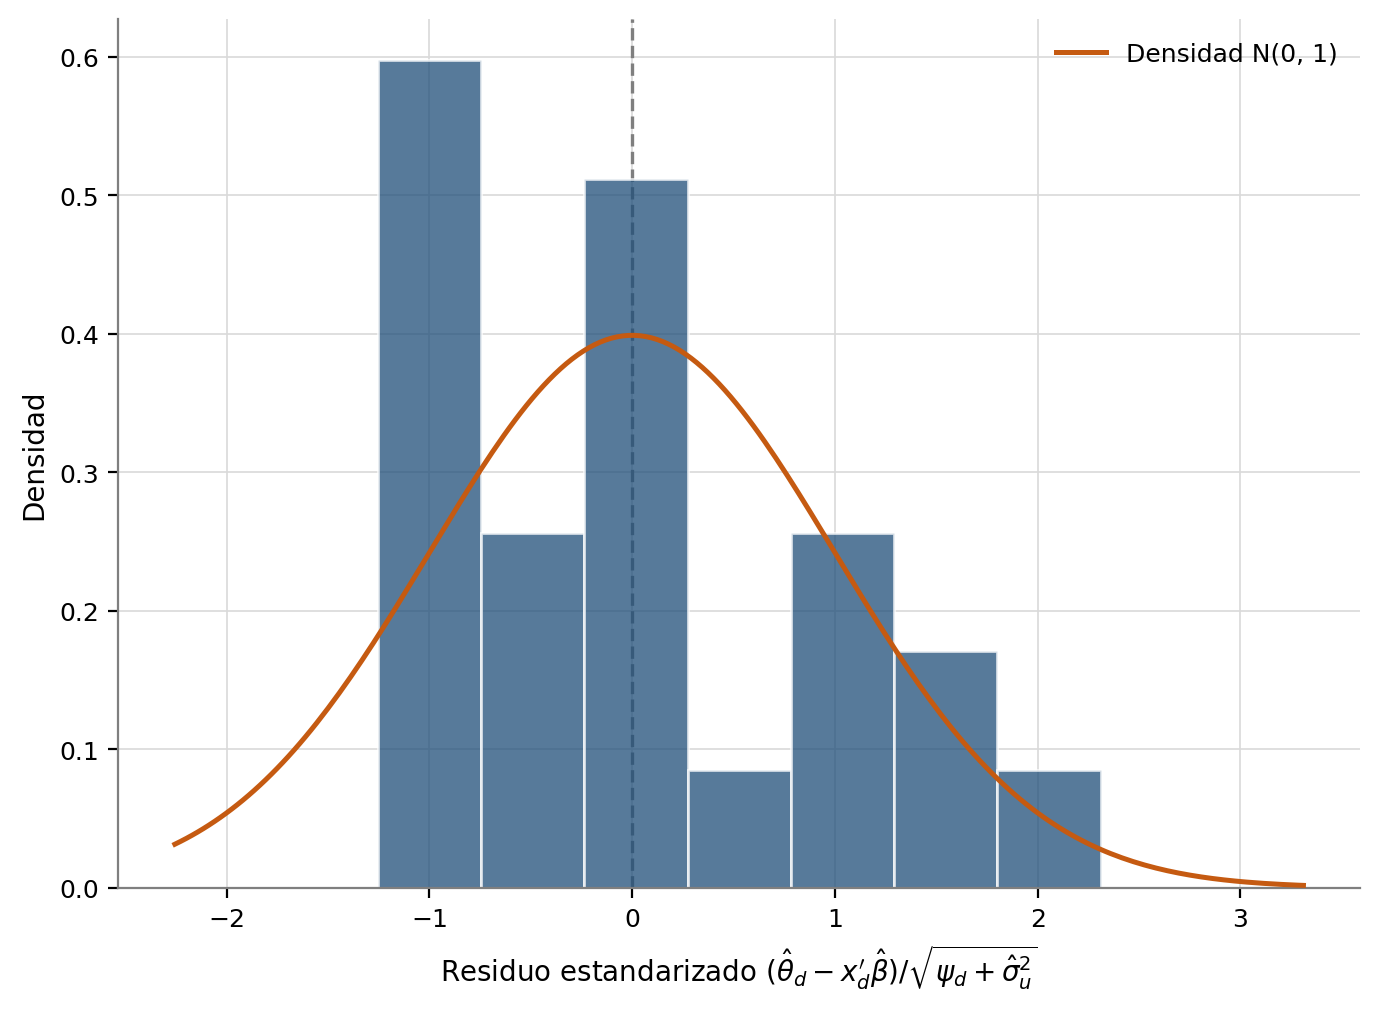
\includegraphics[width=0.48\linewidth]{img/fh_ec0_histograma.png}
\caption{Especificación EC0: a la izquierda, residuo del EBLUP frente a la tasa directa (contracción); a la derecha, histograma de los residuos estandarizados. Fuente: cuaderno del Fay-Herriot clásico.}
\label{fig:app_ec0}
\end{figure}
\begin{figure}[!htbp]
\centering
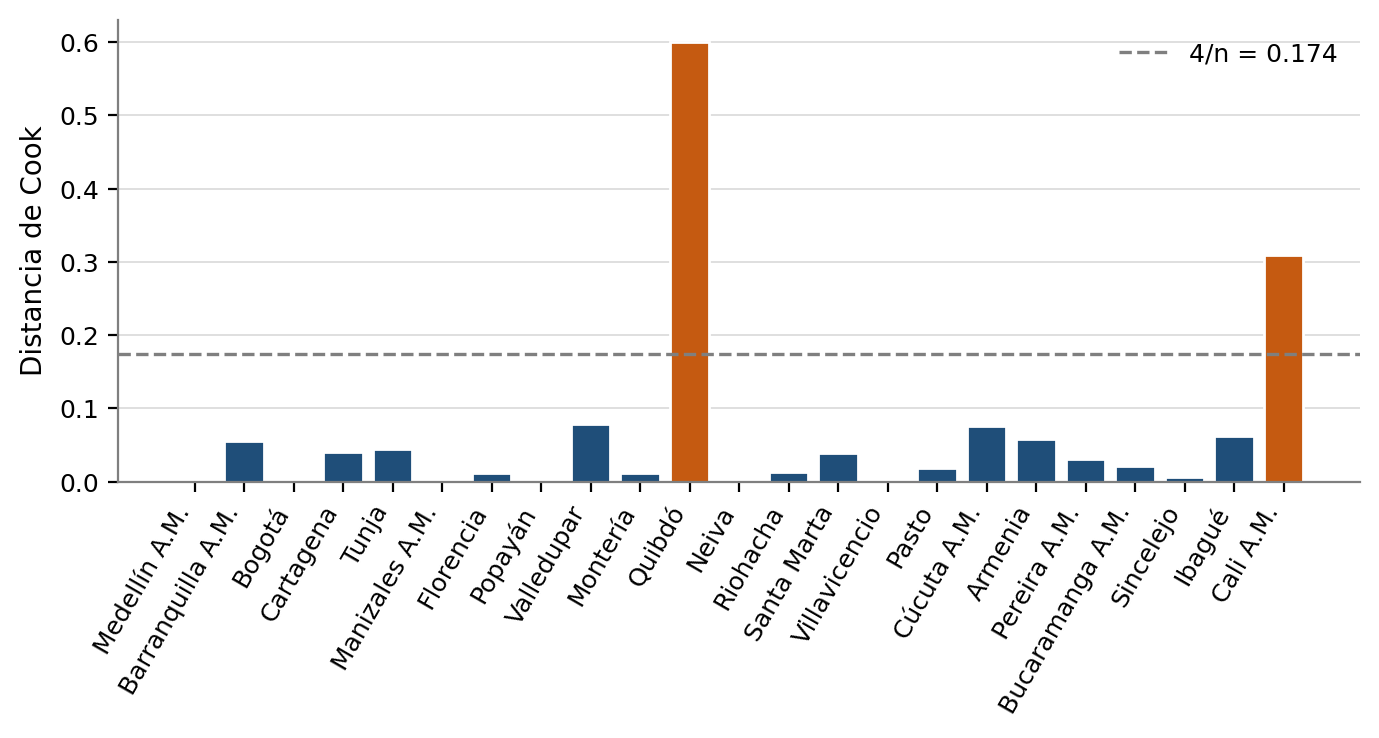
\includegraphics[width=0.85\linewidth]{img/fh_ganador_cook.png}
\caption{Distancia de Cook de cada dominio en el benchmark; la línea marca $4/n$. Fuente: tabla de Cook del Fay-Herriot clásico.}
\label{fig:app_cook}
\end{figure}
\FloatBarrier

%--------------------------------------------------------------------------------------
\anexo{Estimaciones de los dominios}
\label{app:dominios_modelo}

Esta sección presenta, para los 23 dominios, la tasa directa, el EBLUP del benchmark, el SEBLUP del escenario espacial de referencia y el EBLUP ajustado por benchmarking; la citan las Secciones~\ref{sec:res_fh_clasico} y~\ref{sec:res_espacial}.

En la Tabla~\ref{tab:app_dominios_modelo} el EBLUP y el SEBLUP se separan de la tasa directa en 0.10 puntos o menos: el peso de la directa, $\hat{\gamma}_d$, está entre 0.966 y 0.993, de modo que en los dominios los dos modelos casi reproducen la estimación directa. El benchmarking de nivel 1 mueve el EBLUP en 0.01 puntos o menos.

{\footnotesize\setlength{\tabcolsep}{3pt}
\begin{longtable}{l r r r r r r r r}
\caption[Estimaciones de los dominios]{Estimaciones de los 23 dominios, Ene-Dic 2018, en \%. CV: coeficiente de variación, en \%; EBLUP: benchmark EC3; SEBLUP: versión espacial del EBLUP, 3 vecinos, estructura completa, con error cuadrático medio por bootstrap paramétrico (tabla del SEBLUP de los dominios del cuaderno espacial); Ajustada: EBLUP tras el benchmarking de nivel 1; A.M.: área metropolitana.}
\label{tab:app_dominios_modelo} \\
\toprule
Dominio & Directa & EBLUP & CV & $\hat{\gamma}_d$ & SEBLUP & CV & $\hat{\gamma}^S_d$ & Ajustada \\
\midrule
\endfirsthead
\multicolumn{9}{l}{\tablename~\thetable{}, continuación} \\
\toprule
Dominio & Directa & EBLUP & CV & $\hat{\gamma}_d$ & SEBLUP & CV & $\hat{\gamma}^S_d$ & Ajustada \\
\midrule
\endhead
\bottomrule
\endlastfoot
Armenia & 15.49 & 15.42 & 2.20 & 0.979 & 15.43 & 2.23 & 0.978 & 15.42 \\
Barranquilla A.M. & 8.15 & 8.17 & 2.48 & 0.993 & 8.18 & 2.38 & 0.991 & 8.17 \\
Bogotá & 10.37 & 10.37 & 2.25 & 0.990 & 10.38 & 2.33 & 0.988 & 10.37 \\
Bucaramanga A.M. & 8.74 & 8.76 & 3.13 & 0.986 & 8.79 & 3.01 & 0.984 & 8.76 \\
Cali A.M. & 11.65 & 11.69 & 2.42 & 0.986 & 11.69 & 2.47 & 0.986 & 11.69 \\
Cartagena & 8.35 & 8.39 & 3.10 & 0.988 & 8.37 & 3.13 & 0.985 & 8.38 \\
Cúcuta A.M. & 15.98 & 15.88 & 2.28 & 0.976 & 15.89 & 2.33 & 0.972 & 15.88 \\
Florencia & 12.94 & 12.90 & 2.85 & 0.976 & 12.90 & 2.77 & 0.976 & 12.90 \\
Ibagué & 13.99 & 13.93 & 2.35 & 0.981 & 13.93 & 2.39 & 0.978 & 13.93 \\
Manizales A.M. & 11.24 & 11.23 & 2.52 & 0.986 & 11.23 & 2.43 & 0.984 & 11.23 \\
Medellín A.M. & 11.84 & 11.83 & 2.01 & 0.990 & 11.83 & 1.92 & 0.988 & 11.83 \\
Montería & 9.47 & 9.49 & 2.78 & 0.987 & 9.47 & 2.72 & 0.985 & 9.48 \\
Neiva & 11.53 & 11.53 & 2.67 & 0.983 & 11.53 & 2.80 & 0.983 & 11.53 \\
Pasto & 8.82 & 8.84 & 3.20 & 0.986 & 8.84 & 3.25 & 0.986 & 8.84 \\
Pereira A.M. & 8.87 & 8.90 & 3.01 & 0.987 & 8.91 & 2.98 & 0.986 & 8.90 \\
Popayán & 10.68 & 10.69 & 2.75 & 0.984 & 10.69 & 2.74 & 0.984 & 10.68 \\
Quibdó & 17.81 & 17.76 & 2.46 & 0.966 & 17.77 & 2.44 & 0.964 & 17.76 \\
Riohacha & 13.88 & 13.86 & 2.31 & 0.982 & 13.85 & 2.39 & 0.979 & 13.86 \\
Santa Marta & 8.32 & 8.35 & 2.78 & 0.990 & 8.35 & 2.88 & 0.989 & 8.34 \\
Sincelejo & 9.61 & 9.62 & 2.60 & 0.989 & 9.60 & 2.60 & 0.987 & 9.61 \\
Tunja & 11.31 & 11.28 & 2.87 & 0.981 & 11.28 & 2.83 & 0.977 & 11.28 \\
Valledupar & 14.45 & 14.38 & 2.27 & 0.981 & 14.37 & 2.29 & 0.977 & 14.38 \\
Villavicencio & 11.87 & 11.87 & 2.67 & 0.982 & 11.88 & 2.89 & 0.979 & 11.86 \\
\end{longtable}
}
%--------------------------------------------------------------------------------------
\anexo{Varianza de muestreo}
\label{app:varianza}

Esta sección presenta las varianzas alternativas de cada dominio y las figuras de la GVF y de los escenarios; la cita la Sección~\ref{sec:res_supuestos}.

La Tabla~\ref{tab:app_varianza} muestra que la varianza del bootstrap por viviendas es mayor que la del bootstrap por personas en 20 de los 23 dominios, con razones entre 0.939 y 1.173, y que la linealización de Taylor queda cerca, con razones entre 0.938 y 1.053. La Figura~\ref{fig:app_gvf} compara la varianza observada con la ajustada por las dos GVF, y la Figura~\ref{fig:app_escenarios_varianza} muestra cuánto se mueve el EBLUP de cada dominio en los ocho escenarios alternativos.

{\footnotesize\setlength{\tabcolsep}{3pt}
\begin{longtable}{l r r r r r}
\caption[Varianza de muestreo por dominio]{Varianza de muestreo por dominio: $\psi_d$ del bootstrap por viviendas (puntos porcentuales al cuadrado) y razones frente a las alternativas: bootstrap por personas, Taylor y las dos funciones generalizadas de varianza, GVF (Ecuación~\ref{eq:gvf}; razón GVF/bootstrap). A.M.: área metropolitana.}
\label{tab:app_varianza} \\
\toprule
Dominio & $\psi_d$ & Viv./pers. & Boot./Taylor & GVF A & GVF B \\
\midrule
\endfirsthead
\multicolumn{6}{l}{\tablename~\thetable{}, continuación} \\
\toprule
Dominio & $\psi_d$ & Viv./pers. & Boot./Taylor & GVF A & GVF B \\
\midrule
\endhead
\bottomrule
\endlastfoot
Armenia & 0.117 & 1.142 & 0.996 & 1.067 & 1.021 \\
Barranquilla A.M. & 0.041 & 1.026 & 1.014 & 1.028 & 1.023 \\
Bogotá & 0.055 & 1.087 & 0.974 & 1.029 & 1.044 \\
Bucaramanga A.M. & 0.076 & 1.154 & 1.041 & 0.901 & 0.876 \\
Cali A.M. & 0.081 & 1.129 & 1.032 & 0.933 & 0.931 \\
Cartagena & 0.068 & 1.005 & 1.008 & 1.010 & 0.977 \\
Cúcuta A.M. & 0.134 & 1.105 & 0.965 & 1.033 & 0.993 \\
Florencia & 0.138 & 1.155 & 1.038 & 0.896 & 0.964 \\
Ibagué & 0.108 & 1.076 & 1.006 & 1.038 & 1.028 \\
Manizales A.M. & 0.081 & 1.036 & 0.996 & 1.088 & 1.099 \\
Medellín A.M. & 0.057 & 1.141 & 1.053 & 0.921 & 0.981 \\
Montería & 0.070 & 0.997 & 0.954 & 1.036 & 1.024 \\
Neiva & 0.096 & 1.109 & 1.010 & 0.948 & 0.961 \\
Pasto & 0.081 & 1.126 & 1.034 & 0.969 & 0.969 \\
Pereira A.M. & 0.072 & 1.173 & 1.010 & 1.007 & 0.990 \\
Popayán & 0.087 & 1.082 & 0.972 & 0.980 & 0.993 \\
Quibdó & 0.193 & 1.145 & 0.995 & 0.985 & 0.975 \\
Riohacha & 0.104 & 1.065 & 0.975 & 0.999 & 0.980 \\
Santa Marta & 0.054 & 0.975 & 0.976 & 1.149 & 1.099 \\
Sincelejo & 0.063 & 1.114 & 1.016 & 1.022 & 1.007 \\
Tunja & 0.106 & 0.939 & 0.938 & 1.025 & 1.115 \\
Valledupar & 0.108 & 1.080 & 0.954 & 1.063 & 1.040 \\
Villavicencio & 0.102 & 1.104 & 1.000 & 0.953 & 0.972 \\
\end{longtable}
}
\begin{figure}[!htbp]
\centering
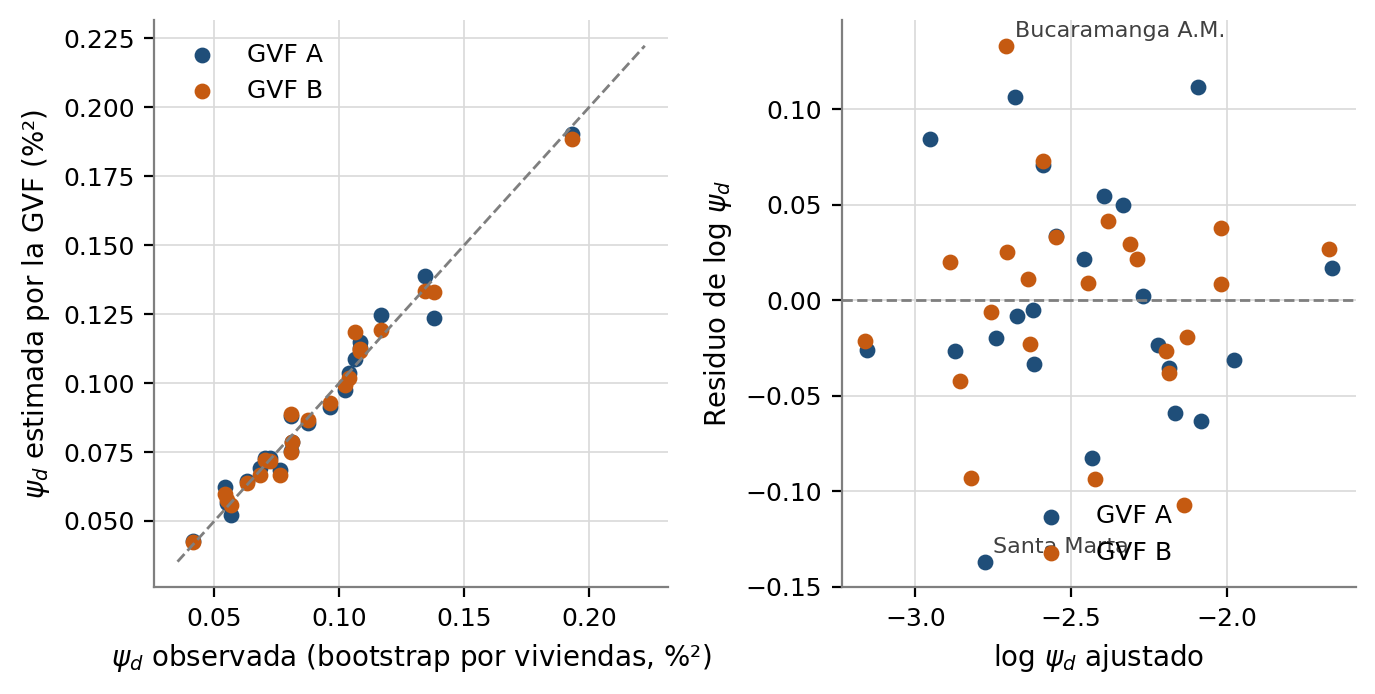
\includegraphics[width=0.9\linewidth]{img/fh_gvf_ajuste.png}
\caption{Varianza de muestreo observada frente a la ajustada por las GVF A y B. Fuente: tabla de ajuste de la GVF.}
\label{fig:app_gvf}
\end{figure}
\begin{figure}[!htbp]
\centering
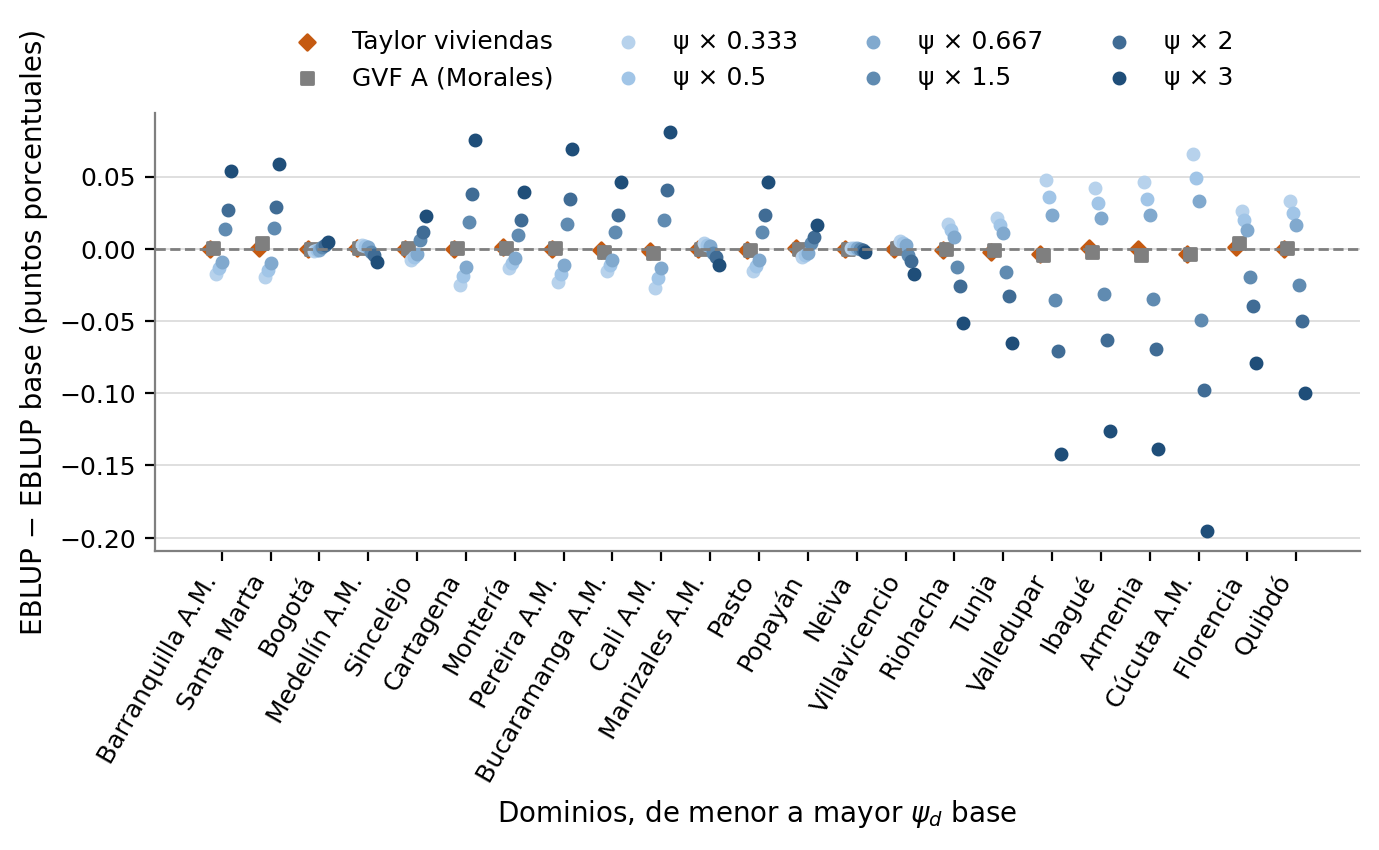
\includegraphics[width=1.0\linewidth]{img/fh_escenarios_varianza.png}
\caption{Cambio del EBLUP de cada dominio frente al escenario base en los ocho escenarios alternativos de la varianza de muestreo. Fuente: tabla de sensibilidad a la varianza por dominio.}
\label{fig:app_escenarios_varianza}
\end{figure}
%--------------------------------------------------------------------------------------
\anexo{Validación predictiva por dominio}
\label{app:validacion}

Esta sección presenta el error de cada dominio retirado en los dos ejercicios de la validación predictiva dejar-un-dominio-fuera; la cita la Sección~\ref{sec:res_validacion}.

En la Tabla~\ref{tab:app_validacion}, con el procedimiento completo el benchmark de cada iteración incluyó la tasa de homicidios en 16 de las 23 y quedó sin covariables en cuatro. Los errores más grandes aparecen cuando el conjunto cambia, como en Armenia ($-7.01$ puntos) y Quibdó ($-6.57$). La Figura~\ref{fig:app_validacion} compara la estimación del dominio retirado con su directa en los dos ejercicios.

{\footnotesize\setlength{\tabcolsep}{3pt}
\begin{longtable}{l r r r r r r r p{2.3cm}}
\caption[Validación predictiva dejar-un-dominio-fuera por dominio]{Validación predictiva dejar-un-dominio-fuera por dominio: estimación sintética del dominio retirado con las covariables fijas y con el procedimiento completo, error frente a la directa (puntos porcentuales) y error estandarizado $Z_{\text{pred}}$. A.M.: área metropolitana.}
\label{tab:app_validacion} \\
\toprule
Dominio & Directa & Fijas & Error & $Z_{\text{pred}}$ & Completo & Error & $Z_{\text{pred}}$ & Covariables (completo) \\
\midrule
\endfirsthead
\multicolumn{9}{l}{\tablename~\thetable{}, continuación} \\
\toprule
Dominio & Directa & Fijas & Error & $Z_{\text{pred}}$ & Completo & Error & $Z_{\text{pred}}$ & Covariables (completo) \\
\midrule
\endhead
\bottomrule
\endlastfoot
Armenia & 15.49 & 11.96 & $-3.53$ & $-1.49$ & 8.48 & $-7.01$ & $-3.17$ & Cobertura neta en educación media \\
Barranquilla A.M. & 8.15 & 11.87 & 3.72 & 1.60 & 11.87 & 3.72 & 1.60 & Tasa de homicidios \\
Bogotá & 10.37 & 10.63 & 0.26 & 0.10 & 5.39 & $-4.98$ & $-1.67$ & Tasa de homicidios, Ingresos tributarios per cápita \\
Bucaramanga A.M. & 8.74 & 10.57 & 1.83 & 0.74 & 10.57 & 1.83 & 0.74 & Tasa de homicidios \\
Cali A.M. & 11.65 & 15.40 & 3.75 & 1.40 & 15.40 & 3.75 & 1.40 & Tasa de homicidios \\
Cartagena & 8.35 & 11.54 & 3.20 & 1.35 & 11.54 & 3.20 & 1.35 & Tasa de homicidios \\
Cúcuta A.M. & 15.98 & 11.62 & $-4.36$ & $-1.90$ & 11.04 & $-4.94$ & $-2.15$ & Cobertura de acueducto \\
Florencia & 12.94 & 11.24 & $-1.70$ & $-0.69$ & 11.46 & $-1.48$ & $-0.52$ & ninguna \\
Ibagué & 13.99 & 10.53 & $-3.47$ & $-1.46$ & 10.53 & $-3.47$ & $-1.46$ & Tasa de homicidios \\
Manizales A.M. & 11.24 & 10.84 & $-0.40$ & $-0.16$ & 10.84 & $-0.40$ & $-0.16$ & Tasa de homicidios \\
Medellín A.M. & 11.84 & 11.42 & $-0.42$ & $-0.17$ & 11.42 & $-0.42$ & $-0.17$ & Tasa de homicidios \\
Montería & 9.47 & 11.11 & 1.64 & 0.67 & 11.11 & 1.64 & 0.67 & Tasa de homicidios \\
Neiva & 11.53 & 11.49 & $-0.04$ & $-0.02$ & 14.35 & 2.82 & 1.07 & Tasa de homicidios, Valor agregado de actividades primarias \\
Pasto & 8.82 & 10.55 & 1.74 & 0.70 & 11.65 & 2.83 & 1.03 & ninguna \\
Pereira A.M. & 8.87 & 11.65 & 2.79 & 1.16 & 11.65 & 2.79 & 1.16 & Tasa de homicidios \\
Popayán & 10.68 & 11.25 & 0.57 & 0.23 & 11.25 & 0.57 & 0.23 & Tasa de homicidios \\
Quibdó & 17.81 & 14.35 & $-3.46$ & $-0.94$ & 11.24 & $-6.57$ & $-2.66$ & ninguna \\
Riohacha & 13.88 & 12.42 & $-1.46$ & $-0.59$ & 11.42 & $-2.46$ & $-0.89$ & ninguna \\
Santa Marta & 8.32 & 11.42 & 3.10 & 1.30 & 12.82 & 4.50 & 1.91 & Cobertura de acueducto \\
Sincelejo & 9.61 & 10.69 & 1.08 & 0.43 & 10.69 & 1.08 & 0.43 & Tasa de homicidios \\
Tunja & 11.31 & 9.34 & $-1.98$ & $-0.77$ & 9.34 & $-1.98$ & $-0.77$ & Tasa de homicidios \\
Valledupar & 14.45 & 10.52 & $-3.93$ & $-1.67$ & 10.52 & $-3.93$ & $-1.67$ & Tasa de homicidios \\
Villavicencio & 11.87 & 11.39 & $-0.48$ & $-0.19$ & 11.39 & $-0.48$ & $-0.19$ & Tasa de homicidios \\
\end{longtable}
}
\begin{figure}[!htbp]
\centering
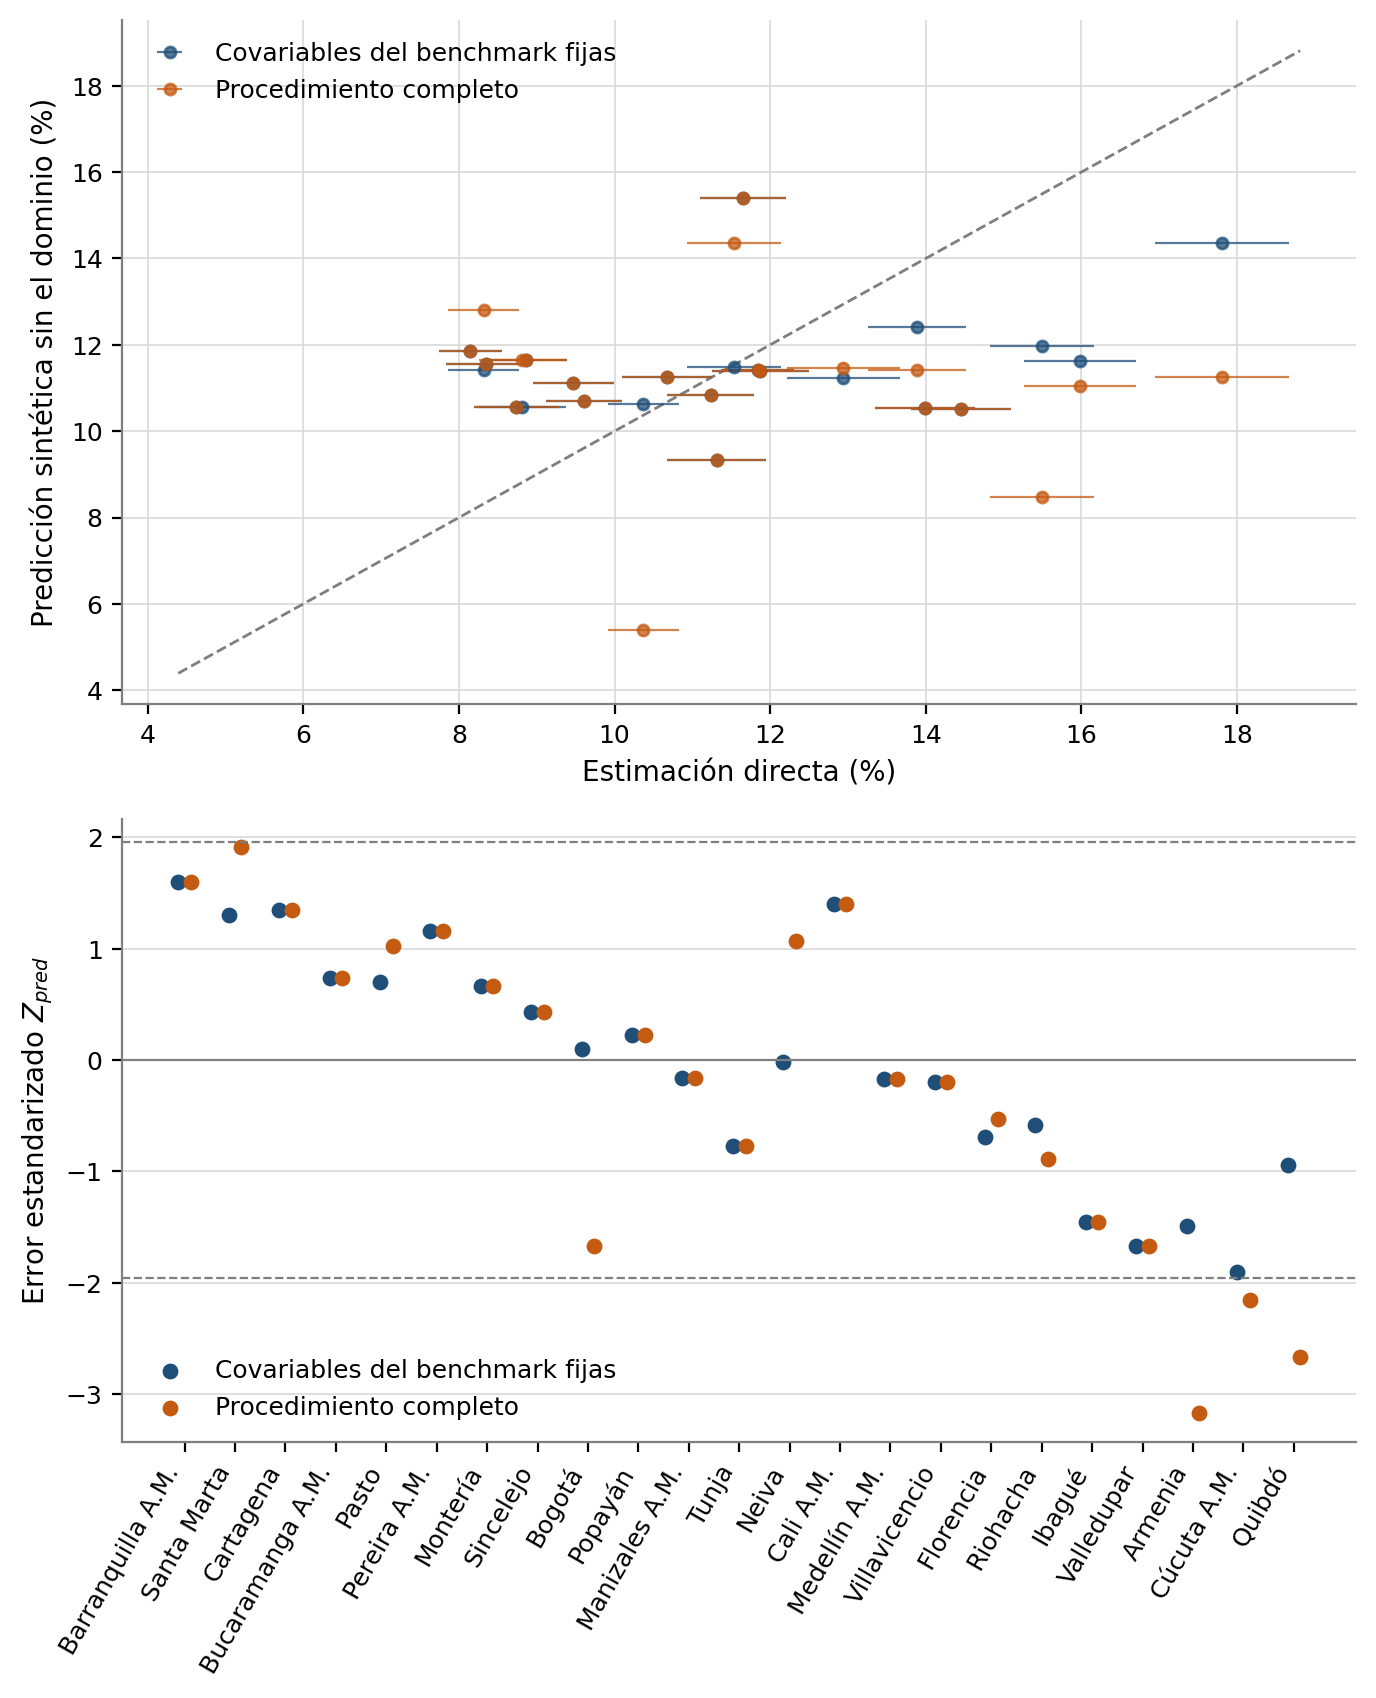
\includegraphics[width=0.9\linewidth]{img/fh_validacion_cruzada.png}
\caption{Estimación del dominio retirado frente a su estimación directa en los dos ejercicios. Fuente: tabla de validación cruzada del Fay-Herriot clásico.}
\label{fig:app_validacion}
\end{figure}
%--------------------------------------------------------------------------------------
\anexo{Detalle del modelo espacial}
\label{app:espacial}

Esta sección presenta las ocho especificaciones espaciales, su validación, sus coeficientes y las sensibilidades del parámetro $\rho$; la cita la Sección~\ref{sec:res_espacial}.

En la Tabla~\ref{tab:app_espacial} ninguna de las ocho especificaciones tiene un LRT con $p < 0.05$ (el menor es 0.221) y todas tienen un AIC mayor que el del clásico. En la validación de la Tabla~\ref{tab:app_espacial_validacion} la RMSE va de 2.35 a 2.86 puntos, frente a 2.52 del sintético clásico, y en la Tabla~\ref{tab:app_espacial_coeficientes} el coeficiente de la tasa de homicidios se mueve menos de 0.13 errores estándar entre especificaciones. Las Tablas~\ref{tab:app_espacial_rho} y~\ref{tab:app_espacial_centroide} muestran que $\hat{\rho}$ de la estructura completa depende de qué municipios entran como nodos y, en menor medida, de dónde se ubica el nodo de cada área metropolitana. Las Figuras~\ref{fig:app_perfil_rho} y~\ref{fig:app_fhe_validacion} presentan el perfil de verosimilitud de $\rho$ y la validación del escenario de referencia.

\begin{table}[!htbp]
\centering
\small
\caption[Especificaciones del Fay-Herriot espacial]{Las ocho especificaciones espaciales con la tasa de homicidios fija. AIC: criterio de información de Akaike; AIC del clásico: 108.904; $\Delta$AIC = AIC clásico $-$ AIC espacial; LRT: estadístico de la prueba de razón de verosimilitudes de $\rho = 0$.}
\label{tab:app_espacial}
\begin{adjustbox}{max width=\linewidth}
\begin{tabular}{l l r r r r r r r}
\toprule
Matriz & Estructura & $\hat{\sigma}_u^2$ & $\hat{\rho}$ & AIC & $\Delta$AIC & LRT & $p$ & $R^2$ \\
\midrule
3 vecinos & muestra & 5.383 & 0.234 & 110.572 & $-1.669$ & 0.331 & 0.565 & 0.268 \\
3 vecinos & completa & 4.825 & 0.372 & 109.403 & $-0.500$ & 1.500 & 0.221 & 0.269 \\
5 vecinos & muestra & 5.541 & 0.206 & 110.901 & $-1.998$ & 0.002 & 0.960 & 0.269 \\
5 vecinos & completa & 5.469 & 0.222 & 110.862 & $-1.958$ & 0.042 & 0.838 & 0.268 \\
Inversa, potencia 1 & muestra & 5.631 & 0.326 & 110.790 & $-1.887$ & 0.113 & 0.737 & 0.269 \\
Inversa, potencia 1 & completa & 5.479 & 0.891 & 110.894 & $-1.990$ & 0.010 & 0.922 & 0.268 \\
Inversa, potencia 2 & muestra & 5.529 & 0.187 & 110.890 & $-1.987$ & 0.013 & 0.909 & 0.269 \\
Inversa, potencia 2 & completa & 5.101 & 0.607 & 110.105 & $-1.201$ & 0.799 & 0.371 & 0.265 \\
\bottomrule
\end{tabular}
\end{adjustbox}
\end{table}
{\footnotesize\setlength{\tabcolsep}{3pt}
\begin{longtable}{p{3.2cm} l r r r r r r}
\caption[Validación del Fay-Herriot espacial por especificación]{Validación dejar-un-dominio-fuera con la tasa de homicidios fija, por especificación y estimador. RMSE: raíz del error cuadrático medio; MAE: error absoluto medio; RMSE$_c$: RMSE corregida por el ruido de muestreo. Errores en puntos porcentuales; Cob.: cobertura del intervalo del 95~\% en \%; habilidad frente al modelo de solo intercepto (RMSE 2.77).}
\label{tab:app_espacial_validacion} \\
\toprule
Especificación & Estimador & RMSE & MAE & Sesgo & RMSE$_c$ & Cob. & Habilidad \\
\midrule
\endfirsthead
\multicolumn{8}{l}{\tablename~\thetable{}, continuación} \\
\toprule
Especificación & Estimador & RMSE & MAE & Sesgo & RMSE$_c$ & Cob. & Habilidad \\
\midrule
\endhead
\bottomrule
\endlastfoot
todos & Sintético clásico & 2.52 & 2.13 & $-0.07$ & 2.51 & 100.00 & 0.17 \\
3 vecinos, muestra & Sintético espacial & 2.53 & 2.12 & $-0.02$ & 2.51 & 100.00 & 0.17 \\
3 vecinos, completa & Sintético espacial & 2.48 & 2.09 & $-0.07$ & 2.46 & 100.00 & 0.20 \\
3 vecinos, completa & Espacial con efecto & 2.35 & 1.99 & $-0.03$ & 2.33 & 100.00 & 0.28 \\
5 vecinos, muestra & Sintético espacial & 2.53 & 2.13 & $-0.10$ & 2.51 & 100.00 & 0.17 \\
5 vecinos, completa & Sintético espacial & 2.52 & 2.12 & $-0.07$ & 2.50 & 100.00 & 0.17 \\
5 vecinos, completa & Espacial con efecto & 2.59 & 2.20 & $-0.02$ & 2.57 & 100.00 & 0.13 \\
Inversa, potencia 1, muestra & Sintético espacial & 2.48 & 2.07 & $-0.25$ & 2.46 & 100.00 & 0.20 \\
Inversa, potencia 1, completa & Sintético espacial & 2.57 & 2.13 & $-0.02$ & 2.55 & 100.00 & 0.14 \\
Inversa, potencia 1, completa & Espacial con efecto & 2.60 & 2.16 & 0.02 & 2.58 & 100.00 & 0.12 \\
Inversa, potencia 2, muestra & Sintético espacial & 2.52 & 2.12 & $-0.03$ & 2.50 & 100.00 & 0.17 \\
Inversa, potencia 2, completa & Sintético espacial & 2.50 & 2.11 & 0.12 & 2.48 & 100.00 & 0.19 \\
Inversa, potencia 2, completa & Espacial con efecto & 2.86 & 2.26 & 0.24 & 2.84 & 91.30 & $-0.06$ \\
\end{longtable}
}
\begin{table}[!htbp]
\centering
\small
\caption[Coeficiente de la tasa de homicidios en el modelo espacial]{Coeficiente de la tasa de homicidios en cada especificación espacial. EE: error estándar. Clásico: 0.099 (EE 0.036, $p = 0.006$); cambio medido en errores estándar del clásico.}
\label{tab:app_espacial_coeficientes}
\begin{tabular}{l l r r r r}
\toprule
Matriz & Estructura & $\hat{\beta}_1$ & EE & $p$ & Cambio en EE \\
\midrule
3 vecinos & muestra & 0.104 & 0.035 & 0.003 & 0.118 \\
3 vecinos & completa & 0.102 & 0.035 & 0.004 & 0.069 \\
5 vecinos & muestra & 0.101 & 0.036 & 0.005 & 0.042 \\
5 vecinos & completa & 0.104 & 0.036 & 0.004 & 0.126 \\
Inversa, potencia 1 & muestra & 0.099 & 0.036 & 0.006 & 0.006 \\
Inversa, potencia 1 & completa & 0.099 & 0.036 & 0.006 & 0.000 \\
Inversa, potencia 2 & muestra & 0.100 & 0.036 & 0.005 & 0.012 \\
Inversa, potencia 2 & completa & 0.099 & 0.035 & 0.005 & $-0.021$ \\
\bottomrule
\end{tabular}
\end{table}
{\footnotesize\setlength{\tabcolsep}{3pt}
\begin{longtable}{l l r r r}
\caption[Sensibilidad de $\hat{\rho}$ a los nodos sin dato]{Sensibilidad de $\hat{\rho}$ de la estructura completa a los municipios objetivo incluidos como nodos.}
\label{tab:app_espacial_rho} \\
\toprule
Matriz & Nodos sin dato & Nodos & $\hat{\rho}$ & $p$ \\
\midrule
\endfirsthead
\multicolumn{5}{l}{\tablename~\thetable{}, continuación} \\
\toprule
Matriz & Nodos sin dato & Nodos & $\hat{\rho}$ & $p$ \\
\midrule
\endhead
\bottomrule
\endlastfoot
3 vecinos & todos & 81 & 0.372 & 0.221 \\
5 vecinos & todos & 81 & 0.222 & 0.838 \\
Inversa, potencia 1 & todos & 81 & 0.891 & 0.922 \\
Inversa, potencia 2 & todos & 81 & 0.607 & 0.371 \\
3 vecinos & solo Valle & 40 & 0.398 & 0.228 \\
5 vecinos & solo Valle & 40 & 0.273 & 0.787 \\
Inversa, potencia 1 & solo Valle & 40 & 0.990 & 0.913 \\
Inversa, potencia 2 & solo Valle & 40 & 0.690 & 0.364 \\
3 vecinos & solo Cauca & 41 & 0.262 & 0.448 \\
5 vecinos & solo Cauca & 41 & 0.157 & 0.947 \\
Inversa, potencia 1 & solo Cauca & 41 & 0.589 & 0.938 \\
Inversa, potencia 2 & solo Cauca & 41 & 0.275 & 0.735 \\
3 vecinos & ninguno & 0 & 0.234 & 0.565 \\
5 vecinos & ninguno & 0 & 0.206 & 0.960 \\
Inversa, potencia 1 & ninguno & 0 & 0.326 & 0.737 \\
Inversa, potencia 2 & ninguno & 0 & 0.187 & 0.909 \\
\end{longtable}
}
\begin{table}[!htbp]
\centering
\small
\caption[Sensibilidad a la ubicación del nodo de cada área metropolitana]{Sensibilidad a la ubicación del nodo de cada área metropolitana: en la capital o en la media de sus municipios.}
\label{tab:app_espacial_centroide}
\begin{tabular}{l l r r r r}
\toprule
Matriz & Estructura & $\hat{\rho}$ capital & $\hat{\rho}$ media & $p$ capital & $p$ media \\
\midrule
3 vecinos & muestra & 0.234 & 0.234 & 0.565 & 0.565 \\
3 vecinos & completa & 0.372 & 0.372 & 0.221 & 0.227 \\
5 vecinos & muestra & 0.206 & 0.278 & 0.960 & 0.767 \\
5 vecinos & completa & 0.222 & 0.353 & 0.838 & 0.522 \\
Inversa, potencia 1 & muestra & 0.326 & 0.403 & 0.737 & 0.788 \\
Inversa, potencia 1 & completa & 0.891 & 0.911 & 0.922 & 0.906 \\
Inversa, potencia 2 & muestra & 0.187 & 0.239 & 0.909 & 0.814 \\
Inversa, potencia 2 & completa & 0.607 & 0.616 & 0.371 & 0.354 \\
\bottomrule
\end{tabular}
\end{table}
\begin{figure}[!htbp]
\centering
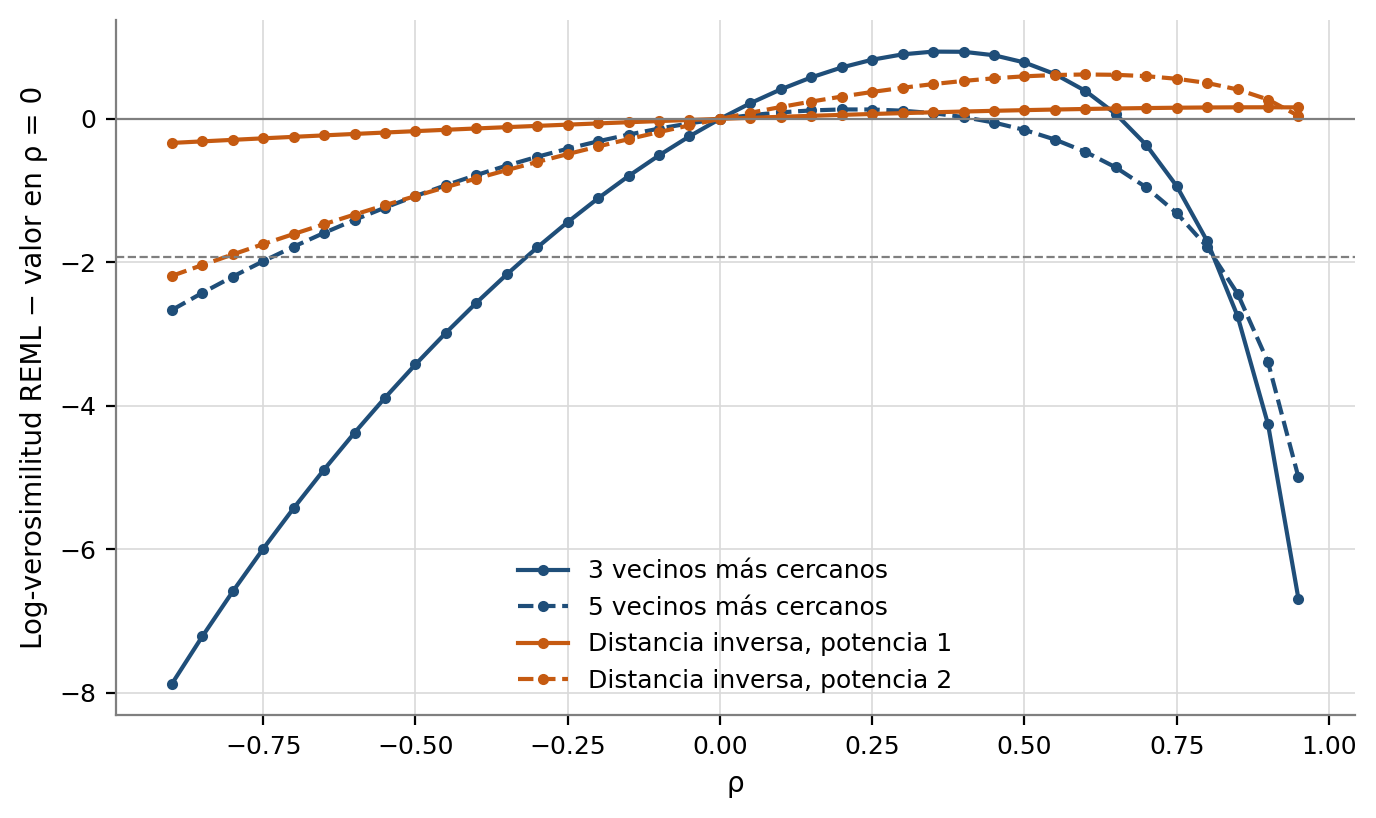
\includegraphics[width=0.85\linewidth]{img/fhe_perfil_rho.png}
\caption{Perfil de verosimilitud de $\rho$ en los cuatro escenarios de la matriz. Fuente: tabla de perfil de $\rho$.}
\label{fig:app_perfil_rho}
\end{figure}
\begin{figure}[!htbp]
\centering
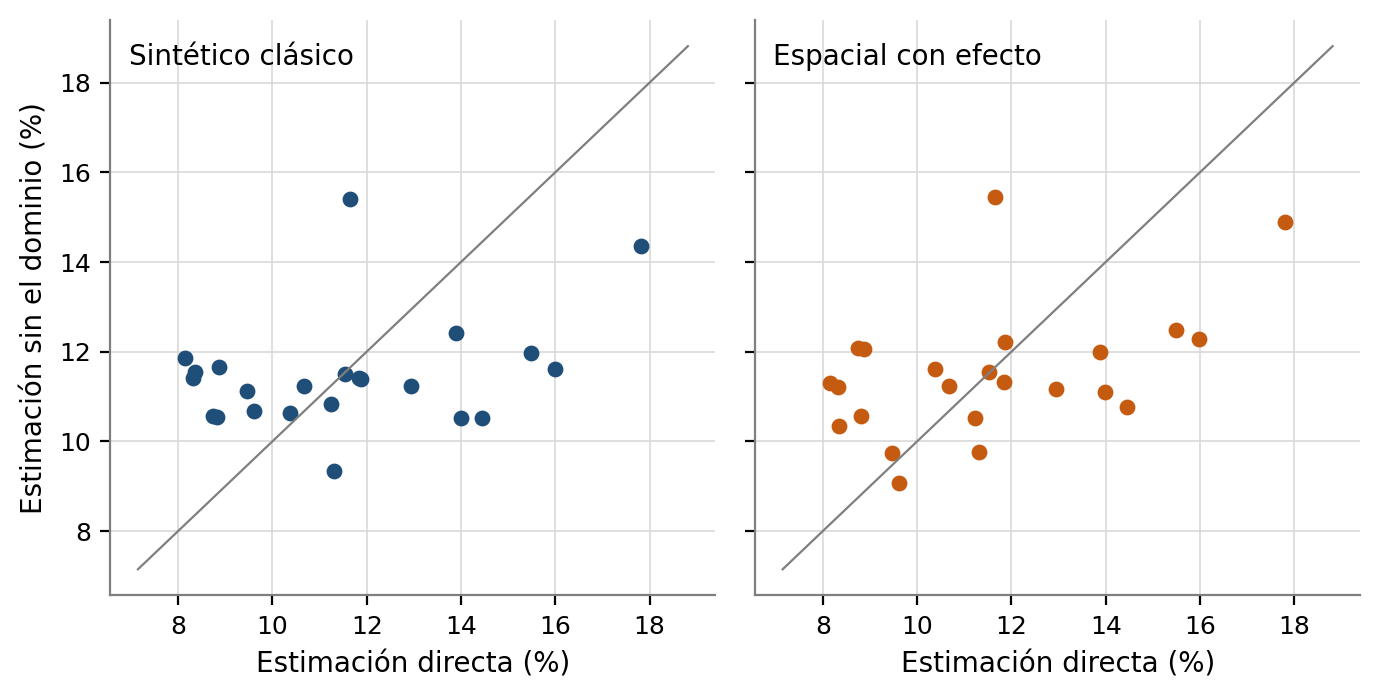
\includegraphics[width=0.9\linewidth]{img/fhe_validacion_cruzada.png}
\caption{Estimación del dominio retirado frente a la directa: sintético clásico y espacial con efecto, escenario de referencia. Fuente: tabla de validación cruzada del modelo espacial.}
\label{fig:app_fhe_validacion}
\end{figure}
\FloatBarrier

%--------------------------------------------------------------------------------------
\anexo{Estimaciones de los 83 municipios}
\label{app:municipios}

Esta sección presenta la estimación de cada municipio objetivo en la tabla final y con el modelo espacial; la citan las Secciones~\ref{sec:res_sin_muestra}, \ref{sec:res_benchmarking} y~\ref{sec:res_patrones}.

En la Tabla~\ref{tab:app_municipios} la estimación final solo difiere de la sintética en Cali y Yumbo, por el benchmarking de nivel 2, y la columna Rango marca los municipios con la tasa de homicidios fuera del rango de los dominios. Para esos municipios, la Figura~\ref{fig:app_sensibilidad_extrapolacion} muestra cuánto cambia la estimación al recortar la covariable al rango y al retirar cada dominio.

{\scriptsize\setlength{\tabcolsep}{2pt}
\begin{longtable}{l p{3.0cm} l r r r l l r r}
\caption[Estimaciones de los 83 municipios objetivo]{Estimaciones de los 83 municipios objetivo, 2018, en \%. Sin ajuste: estimación sintética del benchmark; Final: tras el benchmarking (solo cambian Cali y Yumbo); CV: coeficiente de variación, en \%; Clase: por el CV final; Rango: estado de extrapolación; Espacial: estimación espacial del escenario de referencia y su CV. Toda estimación es condicional al modelo.}
\label{tab:app_municipios} \\
\toprule
Código & Municipio & Depto. & Sin ajuste & Final & CV & Clase & Rango & Espacial & CV \\
\midrule
\endfirsthead
\multicolumn{10}{l}{\tablename~\thetable{}, continuación} \\
\toprule
Código & Municipio & Depto. & Sin ajuste & Final & CV & Clase & Rango & Espacial & CV \\
\midrule
\endhead
\bottomrule
\endlastfoot
19022 & Almaguer & Cauca & 14.57 & 14.57 & 18.15 & Aceptable & dentro & 14.59 & 18.78 \\
19050 & Argelia & Cauca & 20.96 & 20.96 & 19.93 & Aceptable & fuera & 21.17 & 20.92 \\
19075 & Balboa & Cauca & 16.71 & 16.71 & 18.25 & Aceptable & fuera & 16.75 & 18.96 \\
19100 & Bolívar & Cauca & 15.45 & 15.45 & 18.07 & Aceptable & dentro & 15.14 & 19.51 \\
19110 & Buenos Aires & Cauca & 16.77 & 16.77 & 18.27 & Aceptable & fuera & 16.87 & 18.53 \\
19130 & Cajibío & Cauca & 12.97 & 12.97 & 18.96 & Aceptable & dentro & 12.88 & 18.84 \\
19137 & Caldono & Cauca & 10.43 & 10.43 & 23.34 & No confiable & dentro & 10.39 & 23.11 \\
19142 & Caloto & Cauca & 17.74 & 17.74 & 18.56 & Aceptable & fuera & 17.84 & 18.86 \\
19212 & Corinto & Cauca & 31.17 & 31.17 & 24.09 & No confiable & fuera & 31.60 & 24.63 \\
19256 & El Tambo & Cauca & 17.66 & 17.66 & 18.53 & Aceptable & fuera & 17.69 & 18.28 \\
19290 & Florencia & Cauca & 13.01 & 13.01 & 18.93 & Aceptable & dentro & 12.59 & 19.61 \\
19300 & Guachené & Cauca & 18.27 & 18.27 & 18.76 & Aceptable & fuera & 18.32 & 18.09 \\
19318 & Guapi & Cauca & 10.99 & 10.99 & 21.94 & No confiable & dentro & 10.95 & 22.37 \\
19355 & Inzá & Cauca & 9.88 & 9.88 & 25.06 & No confiable & dentro & 10.14 & 24.77 \\
19364 & Jambaló & Cauca & 10.86 & 10.86 & 22.23 & No confiable & dentro & 10.84 & 21.05 \\
19392 & La Sierra & Cauca & 11.96 & 11.96 & 20.13 & No confiable & dentro & 11.95 & 20.79 \\
19397 & La Vega & Cauca & 10.41 & 10.41 & 23.42 & No confiable & dentro & 10.40 & 23.93 \\
19418 & López & Cauca & 15.07 & 15.07 & 18.08 & Aceptable & dentro & 15.12 & 17.49 \\
19450 & Mercaderes & Cauca & 16.19 & 16.19 & 18.14 & Aceptable & dentro & 15.85 & 19.08 \\
19455 & Miranda & Cauca & 15.84 & 15.84 & 18.10 & Aceptable & dentro & 15.88 & 18.28 \\
19473 & Morales & Cauca & 11.49 & 11.49 & 20.91 & No confiable & dentro & 11.45 & 20.55 \\
19513 & Padilla & Cauca & 12.19 & 12.19 & 19.81 & Aceptable & dentro & 12.07 & 20.58 \\
19532 & Patía & Cauca & 20.50 & 20.50 & 19.72 & Aceptable & fuera & 20.70 & 20.37 \\
19533 & Piamonte & Cauca & 11.44 & 11.44 & 21.00 & No confiable & dentro & 11.88 & 20.54 \\
19548 & Piendamó & Cauca & 11.14 & 11.14 & 21.61 & No confiable & dentro & 11.10 & 22.07 \\
19573 & Puerto Tejada & Cauca & 24.46 & 24.46 & 21.52 & No confiable & fuera & 24.08 & 20.78 \\
19585 & Puracé & Cauca & 9.19 & 9.19 & 27.71 & No confiable & fuera & 9.01 & 28.06 \\
19517 & Paéz & Cauca & 10.71 & 10.71 & 22.61 & No confiable & dentro & 10.73 & 22.96 \\
19622 & Rosas & Cauca & 12.65 & 12.65 & 19.26 & Aceptable & dentro & 12.63 & 20.83 \\
19693 & San Sebastián & Cauca & 10.10 & 10.10 & 24.34 & No confiable & dentro & 10.10 & 24.32 \\
19701 & Santa Rosa & Cauca & 11.05 & 11.05 & 21.80 & No confiable & dentro & 11.39 & 20.81 \\
19698 & Santander de Quilichao & Cauca & 15.21 & 15.21 & 18.07 & Aceptable & dentro & 15.27 & 18.65 \\
19743 & Silvia & Cauca & 9.19 & 9.19 & 27.71 & No confiable & fuera & 9.16 & 28.64 \\
19760 & Sotará & Cauca & 11.33 & 11.33 & 21.22 & No confiable & dentro & 11.27 & 22.10 \\
19785 & Sucre & Cauca & 11.28 & 11.28 & 21.31 & No confiable & dentro & 11.26 & 21.42 \\
19780 & Suárez & Cauca & 16.66 & 16.66 & 18.24 & Aceptable & fuera & 16.76 & 18.34 \\
19809 & Timbiquí & Cauca & 14.52 & 14.52 & 18.16 & Aceptable & dentro & 14.57 & 18.55 \\
19807 & Timbío & Cauca & 11.43 & 11.43 & 21.03 & No confiable & dentro & 11.30 & 21.29 \\
19821 & Toribío & Cauca & 10.60 & 10.60 & 22.89 & No confiable & dentro & 10.55 & 23.14 \\
19824 & Totoró & Cauca & 11.21 & 11.21 & 21.45 & No confiable & dentro & 11.22 & 20.97 \\
19845 & Villa Rica & Cauca & 17.34 & 17.34 & 18.43 & Aceptable & fuera & 17.24 & 17.88 \\
76020 & Alcalá & Valle & 13.43 & 13.43 & 18.62 & Aceptable & dentro & 14.01 & 16.46 \\
76036 & Andalucía & Valle & 17.60 & 17.60 & 18.51 & Aceptable & fuera & 17.73 & 19.13 \\
76041 & Ansermanuevo & Valle & 20.00 & 20.00 & 19.49 & Aceptable & fuera & 20.22 & 18.36 \\
76054 & Argelia & Valle & 20.23 & 20.23 & 19.59 & Aceptable & fuera & 20.71 & 18.50 \\
76100 & Bolívar & Valle & 16.01 & 16.01 & 18.12 & Aceptable & dentro & 16.12 & 18.10 \\
76109 & Buenaventura & Valle & 12.12 & 12.12 & 19.90 & Aceptable & dentro & 12.12 & 20.66 \\
76113 & Bugalagrande & Valle & 15.72 & 15.72 & 18.09 & Aceptable & dentro & 15.82 & 18.88 \\
76122 & Caicedonia & Valle & 15.73 & 15.73 & 18.09 & Aceptable & dentro & 16.53 & 17.34 \\
76126 & Calima & Valle & 11.94 & 11.94 & 20.16 & No confiable & dentro & 11.93 & 20.11 \\
76130 & Candelaria & Valle & 15.57 & 15.57 & 18.08 & Aceptable & dentro & 15.02 & 17.23 \\
76147 & Cartago & Valle & 12.55 & 12.55 & 19.37 & Aceptable & dentro & 12.20 & 19.87 \\
76233 & Dagua & Valle & 11.85 & 11.85 & 20.29 & No confiable & dentro & 11.84 & 19.67 \\
76246 & El Cairo & Valle & 10.64 & 10.64 & 22.78 & No confiable & dentro & 10.89 & 22.31 \\
76248 & El Cerrito & Valle & 16.05 & 16.05 & 18.12 & Aceptable & dentro & 16.12 & 18.43 \\
76250 & El Dovio & Valle & 13.66 & 13.66 & 18.48 & Aceptable & dentro & 13.70 & 18.74 \\
76243 & El Águila & Valle & 27.02 & 27.02 & 22.59 & No confiable & fuera & 27.65 & 21.54 \\
76275 & Florida & Valle & 12.30 & 12.30 & 19.66 & Aceptable & dentro & 12.18 & 19.74 \\
76306 & Ginebra & Valle & 9.19 & 9.19 & 27.71 & No confiable & fuera & 9.11 & 28.02 \\
76318 & Guacarí & Valle & 19.36 & 19.36 & 19.21 & Aceptable & fuera & 19.53 & 19.31 \\
76111 & Guadalajara de Buga & Valle & 14.72 & 14.72 & 18.12 & Aceptable & dentro & 14.78 & 18.23 \\
76364 & Jamundí & Valle & 15.65 & 15.65 & 18.08 & Aceptable & dentro & 14.91 & 17.15 \\
76377 & La Cumbre & Valle & 11.02 & 11.02 & 21.87 & No confiable & dentro & 10.98 & 22.12 \\
76400 & La Unión & Valle & 14.75 & 14.75 & 18.11 & Aceptable & dentro & 14.82 & 18.13 \\
76403 & La Victoria & Valle & 15.71 & 15.71 & 18.08 & Aceptable & dentro & 15.81 & 18.35 \\
76497 & Obando & Valle & 14.83 & 14.83 & 18.10 & Aceptable & dentro & 14.86 & 18.04 \\
76520 & Palmira & Valle & 13.62 & 13.62 & 18.50 & Aceptable & dentro & 13.52 & 18.98 \\
76563 & Pradera & Valle & 15.03 & 15.03 & 18.08 & Aceptable & dentro & 14.95 & 17.62 \\
76606 & Restrepo & Valle & 11.78 & 11.78 & 20.40 & No confiable & dentro & 11.77 & 20.69 \\
76616 & Riofrío & Valle & 11.74 & 11.74 & 20.47 & No confiable & dentro & 11.73 & 22.30 \\
76622 & Roldanillo & Valle & 11.62 & 11.62 & 20.68 & No confiable & dentro & 11.62 & 21.01 \\
76670 & San Pedro & Valle & 13.29 & 13.29 & 18.71 & Aceptable & dentro & 13.32 & 19.78 \\
76001 & Cali & Valle & 14.36 & 11.60 & 29.96 & No confiable & dentro & 11.57 & 21.35 \\
76736 & Sevilla & Valle & 11.55 & 11.55 & 20.81 & No confiable & dentro & 11.67 & 21.16 \\
76823 & Toro & Valle & 18.70 & 18.70 & 18.93 & Aceptable & fuera & 18.92 & 18.88 \\
76828 & Trujillo & Valle & 11.26 & 11.26 & 21.36 & No confiable & dentro & 11.23 & 23.10 \\
76834 & Tuluá & Valle & 13.90 & 13.90 & 18.36 & Aceptable & dentro & 13.95 & 17.82 \\
76845 & Ulloa & Valle & 12.82 & 12.82 & 19.09 & Aceptable & dentro & 13.49 & 17.13 \\
76863 & Versalles & Valle & 11.92 & 11.92 & 20.19 & No confiable & dentro & 11.96 & 21.43 \\
76869 & Vijes & Valle & 9.97 & 9.97 & 24.75 & No confiable & dentro & 9.91 & 24.38 \\
76890 & Yotoco & Valle & 11.05 & 11.05 & 21.80 & No confiable & dentro & 11.02 & 22.15 \\
76892 & Yumbo & Valle & 16.96 & 13.70 & 30.03 & No confiable & fuera & 14.24 & 20.72 \\
76895 & Zarzal & Valle & 14.40 & 14.40 & 18.19 & Aceptable & dentro & 14.56 & 17.83 \\
\end{longtable}
}
\begin{figure}[!htbp]
\centering
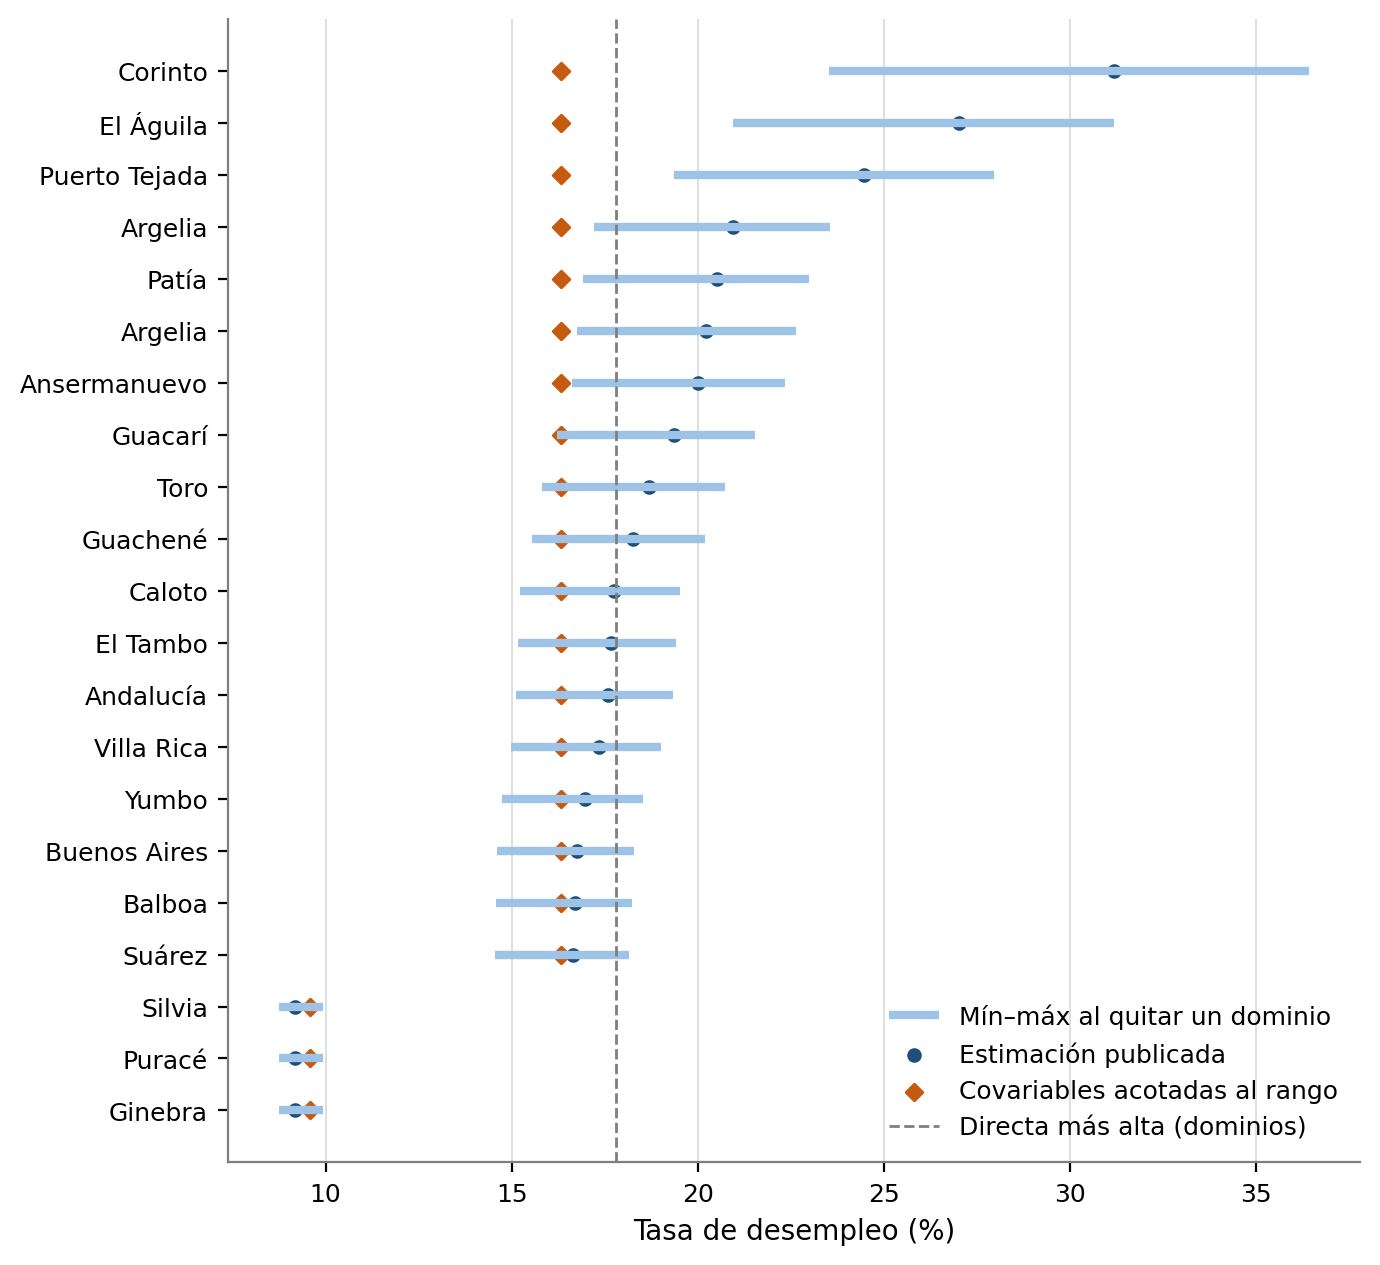
\includegraphics[width=0.9\linewidth]{img/fh_sensibilidad_extrapolacion.png}
\caption{Municipios que extrapolan: estimación publicada, estimación con la tasa de homicidios recortada al rango de los dominios y franja de la estimación al retirar cada dominio. Fuente: tabla de sensibilidad de la extrapolación.}
\label{fig:app_sensibilidad_extrapolacion}
\end{figure}
%--------------------------------------------------------------------------------------
\anexo{Material complementario de Resultados}
\label{app:resultados}

Esta sección reúne tablas de apoyo de la Sección~\ref{sec:resultados} que no responden por sí solas a un objetivo; cada una se cita desde la sección de Resultados que complementa.

\subsection{Tratamiento de faltantes y atípicos}

Complementa la Sección~\ref{sec:res_faltantes}.

\begin{table}[!htbp]
\centering
\small
\caption{Resultado del tratamiento de faltantes y atípicos.}
\label{tab:res_faltantes}
\begin{tabularx}{\linewidth}{>{\raggedright\arraybackslash}p{4.6cm} >{\raggedright\arraybackslash}X}
\toprule
Caso & Resultado \\
\midrule
Factor de expansión faltante & 0 personas; el procesamiento no se detuvo \\
Registros sin código de área & \num{152314} personas de 2018 (762,753 menos 610,439 con área) no se usan; 9 capitales no tienen registros con código de área en 2018 \\
Indicadores de TerriData con faltantes en los dominios & \num{1073} de \num{1582}; salen en el pre-filtrado \\
Candidatas con faltantes en los municipios objetivo & 0 de 18 \\
Valores atípicos en las candidatas (regla del diagrama de caja) & 22 casos en 13 de las 18; Quibdó y Riohacha son los dominios que más se repiten; ninguno se eliminó \\
Valores atípicos en la tasa directa & Ninguno \\
\bottomrule
\end{tabularx}
\end{table}

\subsection{Variables de la literatura sin dato utilizable}

Complementa la Sección~\ref{sec:res_covariables}.

\begin{table}[!htbp]
\centering
\small
\caption{Variables de la revisión de literatura sin dato utilizable.}
\label{tab:res_excluidas}
\begin{tabularx}{\linewidth}{>{\raggedright\arraybackslash}p{5.2cm} >{\raggedright\arraybackslash}X}
\toprule
Variable & Motivo \\
\midrule
Tasa de analfabetismo (censo) & Sin dato en los dominios con encuesta para 2018 \\
Empresas generadoras de empleo formal por cada 10,000 habitantes & La serie termina en 2016 \\
Incidencia de la pobreza monetaria & Solo departamentos y 23 ciudades; no existe en los municipios objetivo \\
Coeficiente de Gini & Solo departamental \\
Víctimas de desplazamiento forzado ubicadas & Solo 2022 y 2023 \\
Índice de incidencia del conflicto armado & Retirado: mide el conflicto en el propio municipio; $r = 0.92$ con la tasa de homicidios en los dominios; 13 valores distintos \\
\bottomrule
\end{tabularx}
\end{table}

\subsection{Sensibilidad de las covariables de las áreas metropolitanas a la regla de agregación}

Complementa la Sección~\ref{sec:res_covariables}.

\begin{table}[!htbp]
\centering
\small
\caption[Sensibilidad de las covariables de las áreas metropolitanas a la regla de agregación]{Cambio relativo máximo en los 7 dominios con área metropolitana (A.M.) entre la agregación con el denominador propio y la agregación con la población de 15 años y más. Solo se muestran las variables con cambio de 1~\% o más; en las otras 14 es menor.}
\label{tab:res_agregacion_am}
\begin{adjustbox}{max width=\linewidth}
\begin{tabular}{l l r l}
\toprule
Covariable & Denominador propio & Cambio máximo (\%) & Dominio \\
\midrule
Densidad de población & Superficie & 67.67 & Bucaramanga A.M. \\
Valor agregado de actividades secundarias & Valor agregado & 43.94 & Cali A.M. \\
Valor agregado de actividades primarias & Valor agregado & 14.23 & Manizales A.M. \\
Valor agregado de actividades terciarias & Valor agregado & 8.04 & Cali A.M. \\
\bottomrule
\end{tabular}
\end{adjustbox}
\end{table}

\subsection{Frecuencia de selección en la validación con el procedimiento completo}

Complementa la Sección~\ref{sec:res_validacion}.

\begin{table}[!htbp]
\centering
\small
\caption{Frecuencia con que cada covariable entra en las 23 iteraciones del procedimiento completo, en la selección de covariables y en el benchmark.}
\label{tab:res_frecuencia}
\begin{tabular}{l r r}
\toprule
Covariable & Selección (\%) & Benchmark (\%) \\
\midrule
Tasa de homicidios & 78.26 & 69.57 \\
Cobertura de acueducto & 56.52 & 8.70 \\
Cobertura neta en educación media & 8.70 & 4.35 \\
Ingresos tributarios per cápita & 4.35 & 4.35 \\
Valor agregado de actividades primarias & 4.35 & 4.35 \\
Ninguna (solo intercepto) & 17.39 & 17.39 \\
\bottomrule
\end{tabular}
\end{table}

\subsection{Validación dejar-un-dominio-fuera del modelo espacial}

Complementa la Sección~\ref{sec:res_espacial}.

\begin{table}[!htbp]
\centering
\small
\caption[Validación del escenario espacial de referencia]{Validación predictiva dejar-un-dominio-fuera con la tasa de homicidios fija, escenario de referencia (3 vecinos, estructura completa). RMSE: raíz del error cuadrático medio; MAE: error absoluto medio. Errores en puntos porcentuales. Las métricas de los cuatro escenarios están en el Apéndice~\ref{app:espacial}.}
\label{tab:res_validacion_espacial}
\begin{adjustbox}{max width=\linewidth}
\begin{tabular}{l r r r r r}
\toprule
Estimador del dominio retirado & RMSE & MAE & Sesgo & Cobertura (\%) & Habilidad \\
\midrule
Sintético clásico & 2.52 & 2.13 & $-0.07$ & 100.00 & 0.17 \\
Sintético espacial & 2.48 & 2.09 & $-0.07$ & 100.00 & 0.20 \\
Espacial con efecto & 2.35 & 1.99 & $-0.03$ & 100.00 & 0.28 \\
Solo intercepto & 2.77 & 2.23 & $-0.01$ & 95.65 & no aplica \\
\bottomrule
\end{tabular}
\end{adjustbox}
\end{table}

\FloatBarrier

